\documentclass[12pt, a4paper, openany]{report}

\def\VersionMemoire{2.0}

\usepackage[utf8]{inputenc} % un package
\usepackage[T1]{fontenc}      % un second package
\usepackage[francais,english]{babel}  % un troisième package
\usepackage{layout}
\usepackage[top=2.7cm, bottom=2.5cm, left=3.5cm, right=3cm]{geometry}
\usepackage{setspace}

\frenchbsetup{StandardLists=true} % à inclure si on utilise \usepackage[french]{babel}
\usepackage{enumitem}
\usepackage{amssymb}

\usepackage{color}
\usepackage{listings}
\definecolor{dkgreen}{rgb}{0,0.6,0}
\definecolor{gray}{rgb}{0.5,0.5,0.5}
\definecolor{mauve}{rgb}{0.58,0,0.82}

\lstset{frame=tb,
  language=Java,
  aboveskip=3mm,
  belowskip=3mm,
  showstringspaces=false,
  columns=flexible,
  basicstyle={\small\ttfamily},
  numbers=none,
  numberstyle=\tiny\color{gray},
  keywordstyle=\color{blue},
  commentstyle=\color{dkgreen},
  stringstyle=\color{mauve},
  breaklines=true,
  breakatwhitespace=true,
  tabsize=3
}

\usepackage{multirow} % pour les tableaux
\usepackage[table]{xcolor} % pour les tableaux

\usepackage{verbatim}
\usepackage{moreverb}
\usepackage{url}
\usepackage{pst-all}
\usepackage{eso-pic,graphicx}
\usepackage{caption} 
\usepackage[colorlinks=true,urlcolor=blue,linkcolor=red]{hyperref}
\usepackage{array}
\usepackage[toc,page]{appendix}
\usepackage[off]{auto-pst-pdf}
\usepackage{hyperref} % pour le sommaire table des matières
\AddThinSpaceBeforeFootnotes % à insérer si on utilise \usepackage[french]{babel}
\FrenchFootnotes % à insérer si on utilise \usepackage[french]{babel}
\usepackage{fancyhdr}
\pagestyle{headings}

\renewcommand{\appendixpagename}{Annexes}
\renewcommand{\appendixtocname}{Annexes}

\title{Memoire: Architecture Microservice}
\author{Lyes \bsc{Kherbiche}}
\date{2016-2017}



%new
\newcommand{\HRule}{\rule{\linewidth}{0.5mm}}


\begin{document}

\selectlanguage{francais}
\pagenumbering{arabic} 

\makeatletter
  \begin{titlepage}
  
  %\centering
   %   {\large \textsc{Université Paris Ouest Nanterre La Défense}}\\
    %  \textsc{SEGMI}\\
    %\vspace{1cm}
     % {\large\textbf{
      %  M2 Miage Classique Nanterre\\
       %\@date}}\\
    %\vfill
    %\vfill
     %  {\LARGE \textbf{\@title}} \\
    %\vspace{2em}
     %   {\large \@author} \\
      %  {\large Tuteur: Mr Fabrice Legon } \\
      
      
      
      
  \begin{sffamily}
   \begin{center}

    % Upper part of the page. The '~' is needed because \\
    % only works if a paragraph has started.
    
\includegraphics[scale=0.5]{parisx.jpg}~\\[1.5cm]

    \textsc{\LARGE UFR SEGMI }\\[2cm]

    \textsc{\Large Mémoire Master II Classique MIAGE}\\[1.5cm]

    % Title
    \HRule \\[0.4cm]
    { \huge \bfseries Architecture Microservice\\[0.4cm] }

    \HRule \\[2cm]
    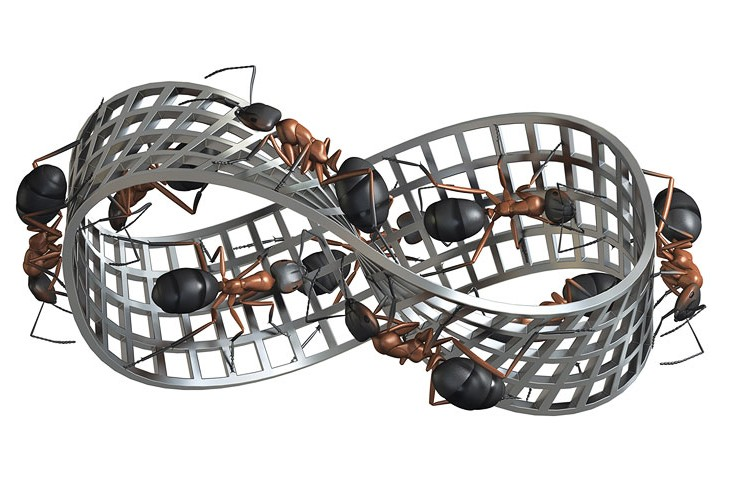
\includegraphics[scale=0.3]{fourmies.jpg}
    \\[2cm]

    % Author and supervisor
    \begin{minipage}{0.4\textwidth}
      \begin{flushleft} \large
         \textsc{Lyes Kherbiche}\\
        Promo 2016-2017\\
      \end{flushleft}
    \end{minipage}
    \begin{minipage}{0.4\textwidth}
      \begin{flushright} \large
        \emph{Tuteur :}  \textsc{M. Legond Fabrice}\\
        \emph{Responsable de la Formation:} \textsc{M. Pascal Poizat}
      \end{flushright}
    \end{minipage}

    \vfill

    % Bottom of the page
    {\large Août 2017}

  \end{center}
  \end{sffamily}      
      
      
      
        
  \end{titlepage}
\makeatother



% *********************** Remerciements *****************
\chapter*{Remerciements}
\addcontentsline{toc}{chapter}{Remerciements}

  Je tiens à exprimer ma profonde gratitude à mon promoteur, monsieur LEGOND pour m'avoir encadré et guidé tout au long de l'année scolaire et mon mémoire, pour ses conseils judicieux et minutieusement prodigués.\\
  
  Aussi je tiens à lui reconnaître le temps précieux qu’il m'a consacré. Mes plus vifs remerciements vont aussi à tout le personnel d'ATOS Rennes plus particulièrement, monsieur Michel Vincent qui m’aide durant mon stage au sien de la société. \\
  
   Que les membres du jury trouvent ici mes remerciements les plus vifs pour avoir accepté d’honorer par leur jugement mon travail.\\
   
   Mes sincères sentiments vont à tous ceux qui, de près ou de loin, ont contribué à la réalisation des mes études supérieurs, en particulier ma chères familles et mes amis (es).\\
   
   
% *********************** Dédicaces *****************
\chapter*{Dédicaces}
\addcontentsline{toc}{chapter}{Dédicaces}
\begin{center}
\begin{Large} \textbf{À mes très chers parents} \end{Large}\\ 
\begin{Large} \textbf{À mes frères} \end{Large}\\
\begin{Large} \textbf{À toute ma famille} \end{Large}\\
\begin{Large} \textbf{À tous mes amis (es)} \end{Large} \\ 
\begin{Large} \textbf{À toute la promo 2016/2017} \end{Large}\\
\end{center}
\begin{flushright} \begin{Large} \textit{Lyes Kherbiche} \end{Large} \end{flushright}

%*********************** somaire **************
\tableofcontents
%*********************** listes des figures **************
\listoffigures
%*********************** listes des tableaux **************
\listoftables



%*********************** INTRODUCTION **************
\chapter*{Introduction}
\addcontentsline{toc}{chapter}{Introduction}
 
  Une des raisons de construire des logiciels est pour une utilité utilisateurs. Il est mieux de faire une application réussie et mal conçue que le contraire, ceci est vrai pour concrétiser l'idée à un artefact qui tourne puis avoir des feedback utilisateurs si la solution est utile avant de se lancer à l’enrichir d'autres besoins utilisateurs. \\
  
  Une fois lancé dans le processus de l’enrichissement, il n'y a pas d'approche formelle à suivre, une multitude de manières de le faire, par contre le concept \textit{monolith first} \footnote{https://martinfowler.com/bliki/MonolithFirst.html} reste une des meilleures façons de procéder au début pour des applications simples.\cite{refbibMonoFirst}. 
  
  Avec le temps, on étend les fonctionnalités existantes et on ajoute d'autres, la quantité de code augmente, plus le temps passe plus les nouvelles fonctionnalités métier deviennent complexes et plus le projet est gros plus les interventions deviennent coûteuses et risquées, on se retrouve dans une impasse qui nous empêche d’évoluer notre système, dans ce cas le monolithe n'arrange pas les choses, d’où le besoin d'une architecture.\\
  
   la science de l’architecture logicielle facilite la modélisation des projets informatiques, elle propose une organisation grossière du système comme une collection de pièces logicielles \cite{refbibFoundations}. L'approche micro-services permet une cadence de développement d'application beaucoup plus rapide.\\
  
  
  Dans ce document, nous nous intéressons à l'architecture basée services notamment l'architecture micro-services (MSA) qui est née dans le web moderne, les micro-services sont interconnectés en utilisant une mince couche d'API simple, de manière générale nous abordons l'architecture logicielle puis les différentes caractéristiques de l'architecture micro-service MSA et une étude comparative de quelques frameworks orientés micro-service.
                                                      



%*********************** Problématique **************
\chapter*{Problématique}
\addcontentsline{toc}{chapter}{Problématique}
   Depuis l’apparition de la nécessité de structurer le code, de l'époque des logiciels monolithiques, les besoins de l'informatique n'ont cessé de croître, l'informatique est divisée en plusieurs disciplines, on trouve notamment l'architecture logicielle, pour acquérir le savoir faire dans cette discipline il faut être sur le terrain, avoir embrassé toute autre discipline et cumuler de l’expérience pour être capable d'affronter ce domaine. \\
   
   Les systèmes informatiques évoluent au fil du temps, ils ne sont jamais stagnés pour éviter d’être obsolètes, car les besoins changent spontanément. La fin des années 90 l'architecture basée services a révolutionné l'industrie informatique, les entreprises adoptent ce nouveau style pour le passage à l’échelle, toucher une variété de domaine, allonger la durée de vie des systèmes et avoir un grand profit business. Plusieurs apparitions de solutions tiers pour aider à mettre en œuvre ce style, les systèmes commencent à grandir, beaucoup d'efforts financiers, humains et techniques sont nécessaires pour maintenir cet élan, ajoutant à cela quelques problèmes connus:
   
    \begin{itemize}[label=$\square$]
      \item  Les applications monolithes de grande taille sont difficiles à maintenir et à évoluer en raison de leur complexité.
      \item  Les problèmes de compilation ou même d’exécution des applications dus à la mise à jour des bibliothèques surtout si elles sont partagées. 
      \item  L'ajout de nouvelles fonctionnalités ou les mises à jour du code nécessite de redéployer toute l'application.
      \item  Les applications monolithiques d'une manière générale sont codées avec un même langage ce qui représente une contrainte technique au développeurs.
  \end{itemize}
  
   Malheureusement beaucoup d'entreprises ont jeté l'éponge à cause de la complication et des coûts colossales, ce qui a poussé de nombreux projets vers l’échec. \\
   
   De nos jours, l'architecture microservice s'affiche pour résoudre certains problèmes des grandes applications encombrées en général et des architectures orientées services en particulier avec son angle de vision, en réduisant la complexité, le temps et la facilité de la mise en marche des applications modulaires et évolutives.
   
   



%*********************** État de l'art **************
\chapter*{État de l'art}
\addcontentsline{toc}{chapter}{État de l'art}
 \chaptermark{État de l'art}

 Les années 1960 ont été le début du développement de logiciels à grande échelle, puis suivi de l'apparition des communautés de recherche sur la conception et son implication sur le développement, juste après, vers les années 1980, l'intégration complète de la conception dans les processus de développement et les références au concept d'architecture de logiciel ont également commencé à apparaître. Vers les années 90 l'architecture logicielle était distincte de la conception de logiciels et depuis lors, une grande communauté de chercheurs s'investissent dans ce domaine qui était adopté par le milieu universitaire (par exemple les travaux de \textit{David Garlan:Software architecture} \cite{refbib4}) et l'entreprise. \\
 
 L'apparition de l'orienté objet a apporté sa propre contribution au domaine de l'architecture de logiciels en définissant des design patterns orientés objet et la séparation des préoccupations qui donnent naissance à l'architecture par composants et par la suite aux SOA\footnote{Service Oriented Architecture}. L'évolution de l'objet vers le service, il existe des différences particulières, le premier est construit au tour de l'idée d'encapsulation et de mémoire partagée, tandis que le second est basé sur l'idée de déploiement des objets distants et qui communiquent par messages.\\
 
 L'architecture orientée service a mis trop d'exigences pour le service comme exemple la découverte et les contrats de services qui sont des contraintes de l'usage de SOA. Les microservices ont vu le jour grâce aux problèmes de SOA, dont l'objectif est de supprimer la complexité inutiles afin de se concentrer sur le développement des services simples qui implémentent chacun une seule fonctionnalité.\\
 
 L'architecture microservices est apparue comme un nouveau paradigme pour la construction d'applications à partir de petits services s'exécutant séparément et communiquant via un mécanisme léger et a été introduit pour la première fois en 2011 \cite{refbibFowler}.  Jusque-là, cette approche avait également été connue sous différents noms par exemple, Netflix a utilisé une architecture très similaire sous le nom de \textit{Fine grained SOA}  \cite{refbibNetflix}.
 
 Maintenant, les microservices sont une nouvelle tendance dans l'architecture de logiciels qui connaissent de plus en plus de popularité au cours des dernières années, tant dans le monde universitaire que dans le monde entreprise. Ils mettent l'accent sur la conception et le développement d'applications hautement scalables et évolutives. Ce style décompose les gros systèmes en un ensemble de services indépendants dans le développement et le déploiement.
 
 Les microservices sont si récents que nous pouvons considérer que leur exploration vient de commencer, la plus grande force des microservices provient de leur distribution ce qui conduit à des systèmes peu couplés. Cependant, de ce même aspect est également la plus grande faiblesse, la programmation des systèmes distribués est plus difficile que les systèmes monolithes, notamment sur la question de prévention des attaques qui exploitent les communications réseau, la gestion des modifications apportées à un service pouvant avoir des effets secondaires sur les autres services avec lesquels il communique, les transactions distribuées et la maturité des langages ou frameworks micro-services. 
 



%*********************** Architecture Logicielle **************
\chapter{Architecture Logicielle}
 L’architecture c’est tout d’abord un art au même titre que la sculpture ou la musique. Il est le premier des arts majeurs et se définit comme l’expression de la culture. Ainsi quand on aborde l’architecture logicielle on devrait plutôt aborder l’ingénierie de construction logicielle.\\ \\
 % captures d’écrans 
 \begin{center}
   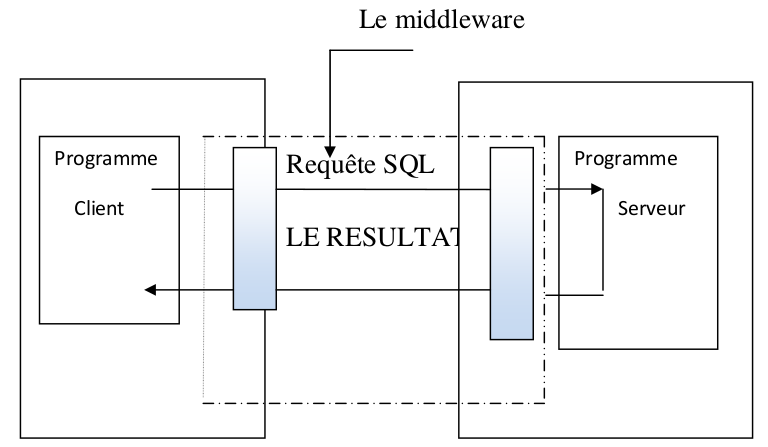
\includegraphics[scale=0.5]{exemple_archi_1.png}
   \captionof{figure}{\textit{Exemple d'architecture}}
   \label{fig1}
 \end{center}
 
 La figure au-dessus a une structure en couches avec des degrés d’implications différents. La partie de gauche interagie avec les utilisateurs, celle de droite traite et persiste des données et enfin la couche du milieu établie les liaisons  et véhicule l’information entre les deux premières.\\
 
 Les logiciels d’entreprise classique, souvent, se représente en multi couches front/back office et décisionnel avec des sous-structure comme composite, fabrique, MVC (Model-View-Controller) implémenter à l’aide de framework, généralement reparties (déployés) sur un ou plusieurs serveurs qui vont communiquer entre elles pour assurer la scalabilité. Ce sont des décisions d’architecture logicielle qui ont leurs avantages et leurs inconvénients.\\
 
 Néanmoins, cette structure n’est jamais stable au fil du temps, elle subit des changements, car elle doit répondre aux nouveaux défis techniques et/ou aux nouveaux besoins des utilisateurs.\\
  
 En court, il y a une différence entre architecture logicielle et celle des bâtiments, si on prend un exemple, la tour Eiffel a toujours la structure et aura la même, tandis que celle d’un logiciel, est fort envisageable qu’elle subira des changements dans le temps.
 
 \paragraph{Définition:}
 L’architecture répond plutôt à la question "Comment le faire" \cite{refbibArch} pour atteindre les objectifs et non pas "que doit doit faire le système" \cite{refbibArch} . D’une autre manière elle décrit comment il doit être construit d’une façon à répondre aux spécifications de l’analyse fonctionnelle.
 
 \section{Évolution de l'architecture}
  Avant les années 80, les architectures des systèmes informatiques étaient centralisées autour de calculateurs centraux (monolithique). Les terminaux étaient passifs, la productivité des développeurs était faible et la maintenance des applications était plus difficile.
  
  Les années 80 ont connu le développement du transactionnel et des bases de données et la nécessité de passer du monobloc vers un assemblage des entités de codes qui collaborent entre eux, ainsi une nouvelle architecture et langage à objet sont nés offrant une certaine granularité.
  
  Cependant, même si l’orienté objet offre une base saine pour le développement d’éléments réutilisables à fine ou à plus grosse granularité \cite{refbib1} , elle n’offre pas les notations adéquates pour la construction à plus large échelle. Les composants constituent des briques de construction à plus large échelle et sont vus comme le prolongement des objets \cite{refbib2}.
  
 À partir des années 90, l’émergence des réseaux a fait naître les applications reparties sous formes de briques distribuées certaines offrent un service et les autres les consomment.

 % captures d’écrans 
   \begin{center}
     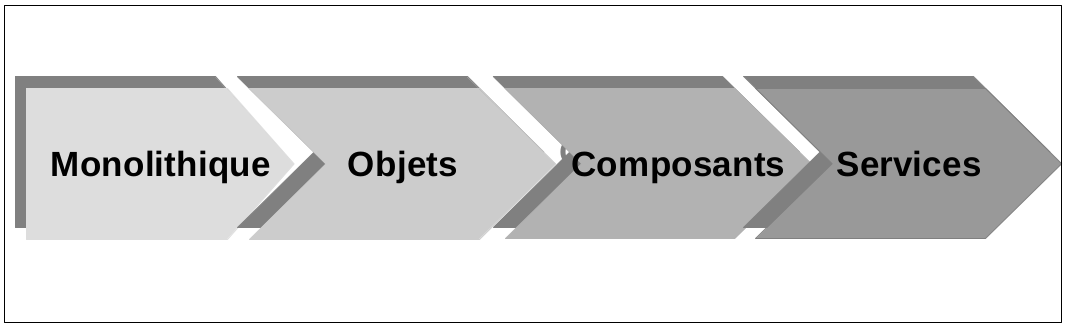
\includegraphics[scale=0.35]{evolution_archi_7.png}
     \captionof{figure}{\textit{Évolution de l'architecture}}
     \label{fig7}
   \end{center}
   
 \section{Pourquoi une architecture logicielle}
 Elle sert toutes les parties prenantes à cerner et comprendre le système, notamment les  développeurs à opérer sur des parties particulières du système, de prévoir à l’avance les endroits susceptibles de modification ou d’extension et favorise la construction de composants réutilisables.
 
 \section{Utilité d’une architecture logicielle} \cite{refbib3}
 
  \begin{itemize}
      \item  Compréhension:
      Facilite la compréhension des grands systèmes complexes en donnant une vue de haut-niveau de leur structure et de leurs contraintes. 
      Les motivation des choix de conception sont ainsi mis en évidence
      \item  Réutilisation:
      Favorise l’identification des éléments réutilisables, parties de conception, composants, caractéristiques, fonctions ou données communes.
      \item  Construction:
      Fournit un plan de haut-niveau du développement et de l’intégration des modules en mettant en évidence les composants, les interactions et les dépendances. Elle doit permettre aux développeurs de travailler sur des parties individuelles du système en isolation.
      \item  Évolution:
      Met en évidence les points où un système peut être modifié et étendu. La séparation composant/connecteur facilite une implémentation du type "plug-and-play".
      \item  Analyse:
      Offre une base pour l’analyse plus approfondie de la conception du logiciel, analyse de la cohérence, test de conformité, analyse des dépendances.
      \item  Gestion:
      Contribue à la gestion générale du projet en permettant aux différentes personnes impliquées de voir comment les différents morceaux du casse-tête seront agencés. L’identification des dépendance entre composants permet d’identifier où les délais peuvent survenir et leur impact sur la planification générale.
  \end{itemize}
  
 \section{Styles d’architectures}
 Un Style architectural est un standard expliquant comment sera le système. Les systèmes ont généralement des ressemblances d’organisation en commun appelés styles architecturaux \cite{refbib4} \footnote{Garlan D. :Software architecture : perspectives on an emerging discipline. Prentice-Hall, Inc., Upper Saddle River, NJ, USA, 1996.}.\\
 
 De plus, un système peut être combiner de plusieurs styles selon les besoins. Quelque des plus courants sont  le style client/serveur, le style Pipe\&Line (tuyau\&filtre), centrée sur les données, le style orienté objet et le style en couches.\\
 
 Les styles architecturaux ont des atouts qui aident à la compréhension pour créer, aussi pour apporter des changements sur le système et les réutiliser (Ne pas réinventer la roue).\\
 
  Citons quelques styles:
  \begin{itemize}
      \item  PipeLine \cite{refbibPipeLine}: ce style est utile pour les logiciels de traitement et de transformation de données par exemple les compilateurs, l'entité filtre reçoit des données en entrées, suivie d'un processus de traitement et de transformation puis redirige les résultats vers une sortie sur un ou plusieurs pipes. L'entité pipe joue le rôle de canal, il connecte deux filtres à travers duquel circulent les données et il est unidirectionnel (figure \ref{fig8}).
 
              % captures d’écrans 
              \begin{center}
                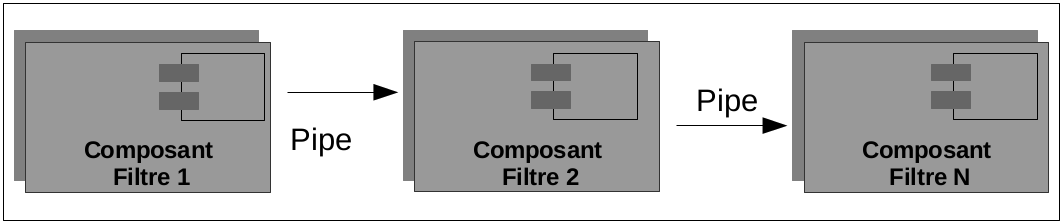
\includegraphics[scale=0.3]{pipe_line_8.png}
                \captionof{figure}{\textit{Style Pipeline}}
                \label{fig8}
              \end{center}
              
      \item  Centrée données: Elle comporte un composant central de type système de gestion de base de données et des composants périphériques, appelés clients, utilisent le composant central appelé serveur de données \cite{refbibCentreDonnee}.
      
      Il est utile dans le cas où des données sont partagées et fréquemment échangées entre les composants, ce style découple les données des traitements, exemple: Oracle Forms \footnote{$http://www.oracle.com/technetwork/developer-tools/forms/overview/index-098877.html$}.
      
      
      \item  couches: Avec ce style, le système est organisé en hiérarchie de couches qui exposent des interfaces bien définies et qui communiquent à travers des protocoles, chaque couche fait l'objet de client ou serveur ou les deux à la fois (figure \ref{fig9}).
             % captures d’écrans 
             \begin{center}
               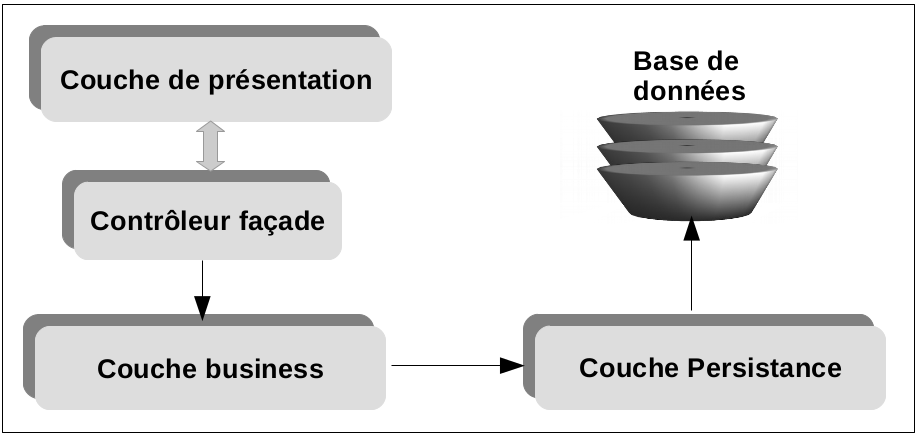
\includegraphics[scale=0.3]{style_couche_9.png}
               \captionof{figure}{\textit{Style en couches}}
               \label{fig9}
             \end{center}
             
  \end{itemize}
  
  
%*********************** MSA **************
\chapter{Architecture Micro-service}
  Microservice Architecture (MSA) se distinguent d'autres architectures notamment l'architecture monolithique, objet, composant et même celles basées services.

    Les Microservice sont des services sous formes de petits composants autonomes qui communiquent ensemble pour réaliser des tâches et ayant un faible couplage \cite{refbibFowler} .  \\

    Le MS pourrait être déployé comme un service isolé en tant que PAAS \footnote{Platform as a service}, cet isolement n'est pas gratuit bien que il rend notre système distribué simple et facile à concevoir en plus de ça, l'avantage des nouvelles technologies qui facilitent les formes de déploiement. Toutes les communications se font à travers le réseau et pour réaliser un faible couplage il faut une bonne modélisation du système d'information et un bon choix des API.
  
    MSA possède des avantages par rapport aux types d'architecture qui partagent des API, des services et possèdent parfois une conception par modules, je cite quelques-uns:  
                                                % itemes
                                                \begin{itemize}
                                                 \item utilisation des technologies hétérogènes .
                                                 \item Elasticité .
                                                 \item Scalabilité .
                                                 \item Facilité de déploiement .
                                                 \item Mise à jour optimale .
                                                \end{itemize}
   
   Dans ce qui suit, j'aborde  
                                                 % itemes
                                                \begin{itemize}
                                                 \item Les architectures basées services .
                                                 \item Les caractéristiques du service .
                                                 \item Les caractéristiques d'architecture .
                                                \end{itemize}
                                                      
 \section{Architectures basées services}
  MSA est une architecture basée service, ses composants mettent de l’importance à la notion de service pour implémenter des fonctionnalités métier et non métier, malgré les différences entre les architectures basées service, elles partagent certaines caractéristiques.\\
 
 Les architectures basées services ont une chose en commun c’est qu’elles sont distribuées, les services que leurs composants offrent, sont accessibles avec des appels distants par exemple, REST (Representational State Transfer), SOAP (Simple Object Access Protocol), AMQP (Advanced Message Queuing Protocol), JMS (Java Message Service), RMI (Remote Method Invocation). Les applications distribuées ont des avantages de scalabilités, de faibles couplages et une maîtrise des processus de développement, de teste et de déploiement, les composants sont presque autonomes et facile à maintenir. Les architectures basées services sont connues d’être modulaire (exemple module maven), la modularité c’est d’encapsuler des parties de l’application en services autonomes chacun est développé, testé et déployé seul avec un minimum de dépendances des autres composants.\\
 
 Les applications distribuées ne sont pas sans exceptions, elles ont des défis à relever, on cite le bon choix du protocole d’accès distant, maintenir le contrat de service, disponibilité de service/gérer les pannes, sécuriser les appels distants, gestion des transactions, tous cela se sont quelques points a ne pas prendre à la légère pour créer des architectures basées service.\\
 
  \subsection{Contrat de service}
  Le contrat de service est un agrément entre le service distant et son consommateur qui est le client et on déclare dedans le format des données qui s’échangent entre eux, XML, Json, des objets java etc. Concevoir un contrat de service n’est pas une chose facile car il faut prévoir à l’avance sa maintenance et ses prochaines versions pour d’autres consommateurs. Exemple : Comme la figure \ref{fig2} au-dessous le montre, on a un service qui expose à ses consommateurs la météo, au début il était conçue de fournir la météo du jour même (Version 1), au fil du temps de nouveaux besoins d’autres utilisateurs apparaissent (Météo sur plusieurs jours), l’idée c’est de maintenir l’ancien service (car il possède encore des consommateurs) et de créer un autre avec le même contrat et du coût on aura plusieurs versions du service.\\
  
  Cette approche de supporter les versions d’un contrat de service permet de développer et de déployer de nouvelles fonctionnalités et d’apporter des changements sans casser les contrats existants avec les consommateurs.\\
  
  % captures d’écrans 
   \begin{center}
     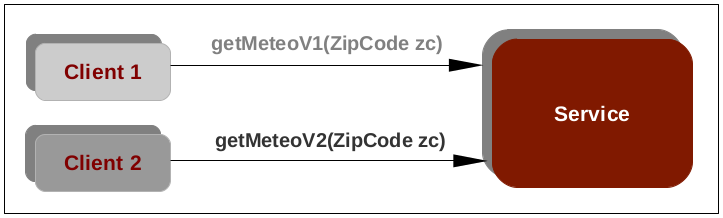
\includegraphics[scale=0.52]{version_contrat_2.png}
     \captionof{figure}{\textit{versions de contrat de service}}
     \label{fig2}
   \end{center}  
  
  \subsection{Réactivité \& Disponibilité de service}
   
   La figure \ref{fig3} illustre la différence entre disponibilité et réactivité de services, ces deux notions ont un rapport direct avec la capacité de communication entre le client et le service distant.
   
   % captures d’écrans 
   \begin{center}
     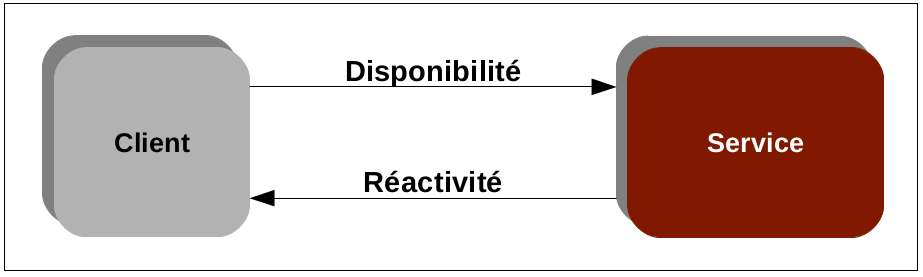
\includegraphics[scale=0.4]{reactivite_disponibilite_service_3.png}
     \captionof{figure}{\textit{réactivité vs disponibilité de service}}
     \label{fig3}
   \end{center}
   
   % itemes
   \begin{itemize}
      \item La disponibilité: fait référence à l’établissement de la connexion et la capacité de répondre au requêtes du client vers le service distant \cite{refbibDispo}.
      \item La réactivité \footnote{https://hal.inria.fr/inria-00177149/document}: fait référence à la réception de la réponse par le demandeur du service dans des délais acceptables. 
  \end{itemize}
  
  À défaut de ces conditions la requête ne sera pas accomplie.
  
  \subsection{Sécurité}
  Il est très important de sécuriser les accès distants, certains services exposés doivent être protégés, en d’autres termes le demandeur doit être authentifié et autorisé.
  % itemes
  \begin{itemize}
      \item authentification\footnote{https://fr.wikipedia.org/wiki/Authentification}: désigne le processus visant à confirmer qu'un commettant est bien légitime pour accéder au système.
      \item autorisation\footnote{https://fr.wikipedia.org/wiki/Autorisation}: est la fonction spécifiant les droits d'accès vers les ressources liées à la sécurité de l'information et la sécurité des systèmes d'information en général et au contrôle d'accès en particulier.
  \end{itemize}
  Les micro-services sont indépendants, en partant de ce concept et laissant la gestion de la sécurité à un service à part, on obtient un fort couplage et une dépendance pour chaque service qu’on doit protéger, autrement dans le cas ou on fabrique des services qui gèrent leurs sécurités on aura énormément de redondance, avec les MSA la sécurité devient un défi, les solutions qui semblent être correctes c’est de déléguer l’authentification à un service dédié et manœuvrer les autorisations au sein même du service.
  
  \subsection{Gestion de données et Transactions}
  Les entreprises préfèrent avoir des bases de données centralisées non fédérées, une base par contexte applicatif, car c’est plus avantageux et plus facile à gérer.

  Avec les MSA Chaque service gère sa propre base de données (illustration figure \ref{fig25}), une décentralisation du schéma physique et logique de données.

  La décentralisation des données entre les micro-services à des implications sur la cohérence des données,  pour palier à cette difficulté , les MS (même les différentes autres architectures) ont recours à des mises à jour entre les différentes ressources de données  qui sont traitées à l’aide des transactions dites distribuées \cite{refbibFowler}.  \\
  
   % captures d’écrans 
   \begin{center}
     %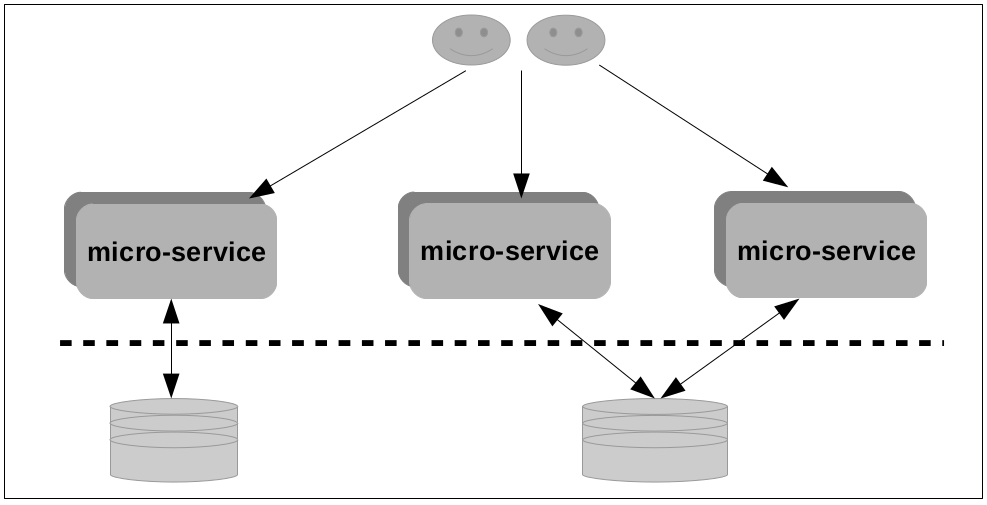
\includegraphics[scale=0.3]{decentra_db_25.png}
     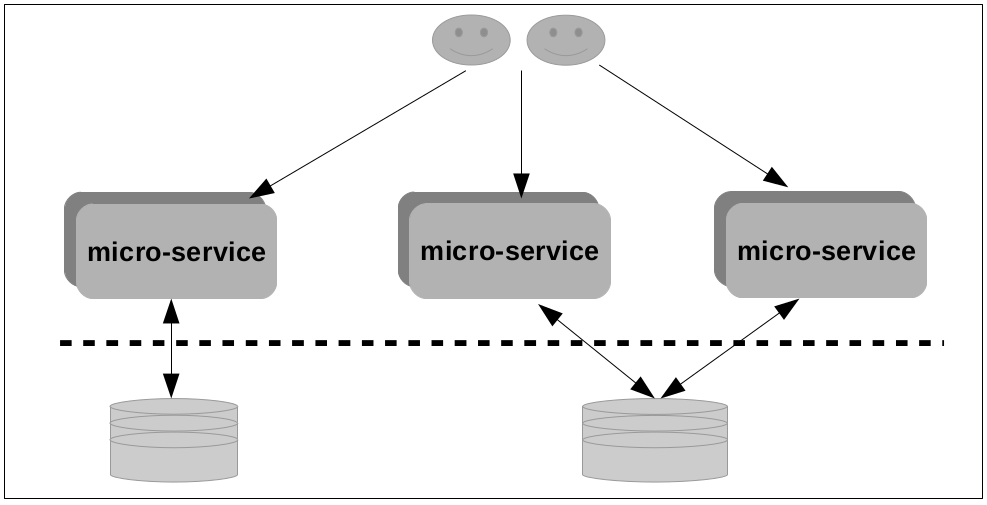
\includegraphics[width=\textwidth, height=5cm]{decentra_db_25.png}
     \captionof{figure}{\textit{Décentralisation des bases de données}}
     \label{fig25}
   \end{center}
  
  Dans le contexte de micro services la mise en œuvre de mécanismes relatifs aux transactions constitue souvent une difficulté, cela s’explique par le faite que souvent les transactions se basent sur les principes suivants (ACID) \footnote{$https://vladmihalcea.com/2014/01/05/a-beginners-guide-to-acid-and-database-transactions/$} \cite{refbibAcid} : 
  
   %itemize
   \begin{itemize}
      \item Atomicité : Un ensemble d’opérations (souvent lecture/écriture) constitue une seule opération qu’on exécute entièrement ou pas du tout. 
      \item Consistance : (Cohérence) Cela implique une cohérence dans les données mais aussi le non échec de tout opération voir sous opération relative aux données (exemple échec de l’exécution d’un trigger de Base de données).
      \item Isolation : On arrive à gérer souvent cela grâce aux mécanismes d’accès concurrents tel que les locks.
      \item Durabilité : est le faite de pouvoir s’assurer qu’au cas du crash d’un système par exemple qu’on puisse rejouer toutes les transactions non achevés. 
   \end{itemize}
   
   Les quatre principes énoncés précédemment deviennent presque un challenge dans le cadre micro-services, les transactions distribuées sont incontestablement difficiles à mettre en œuvre, car une transaction fera plusieurs appels distants à différentes ressources de données des micro services, de ce faite les transactions dans le cadre de micro-services à un moment la cohérence est partielle, les données seront cohérentes qu’après un laps de temps après  la transaction.
   
     Pour conclure sur ce point on peut dire que dans le cadre des transactions micro services il faut sortir du principe classique ACID et prendre en compte un laps de temps pour la cohérence, ce principe est une alternative, c'est les transactions BASE \footnote{$http://www.dataversity.net/acid-vs-base-the-shifting-ph-of-database-transaction-processing/$} \cite{refbibBase}: 
     %itemize
   \begin{itemize}
      \item Basic Availability: La base de données semble fonctionner la plupart du temps, le système est disponible, mais pas nécessairement toutes ressources à un moment donné.
      \item Soft-state: L'état du système pourrait changer avec le temps, de sorte que, même en période sans activités, il se peut qu'il y ait des changements en raison de la cohérence partielles, donc l'état du système est toujours doux.
      \item Eventual consistency: Après un certain laps de temps, toutes les sources de données sont cohérentes, mais à tout moment, cela pourrait ne pas être le cas.
   \end{itemize} 
   
 
 \section{Caractéristiques du service}
  \subsection{Classification de service}
   La classification dans l’ensemble de l’architecture s’attribue au type/rôle du service d’un coté et le domaine métier de l’autre.
   
   On entend par type l’implantation fonctionnelle ou non fonctionnelle et par métier (business) le cœur, le but, la finalité du service, exemple faire une réservation, insertion d'un client.\\
   
   En analogie aux SOA comme le montre la figure \ref{fig4}, on trouve une variété de rôle/type de service, la pattern d'architecture SOA exige une définition de quatre types/rôles: Service métier, entreprise, application et à la fin le service infrastructure.
   %itemize
   \begin{itemize}
      \item  Service métier: est quelque chose d’abstrait il a des entrées et sorties mais il implante pas le cœur métier car il porte juste le nom du service , son rôle par exemple la vérification/validation des données d’entré (primitifs, XML, etc) et il aiguille vers le service d'entreprise adéquat.
      \item  Service entreprise: est partagé par la majorité de l'organisation, c'est à ce niveau que se fait l'implantation effectif des fonctionnalités définies dans service métier, il utilise la brique middleware comme intermédiaire entre les service métier abstrait et son relatif effectif.
      \item  Service application:c'est comme le service entreprise on trouve l'implantation fonctionnelle à la différence il n'est pas partagé en d'autre termes il contient des fonctions spécifiques.
      \item  Service infrastructure: il englobe le non fonctionnel, exemple Log, sécurité, performances ...  
   \end{itemize}
    
   % captures d’écrans 
   \begin{center}
     %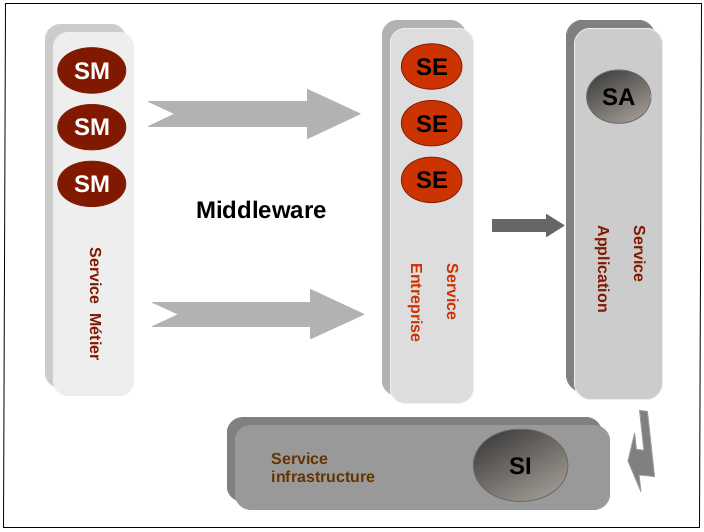
\includegraphics[scale=0.35]{classif_soa_4.png}
     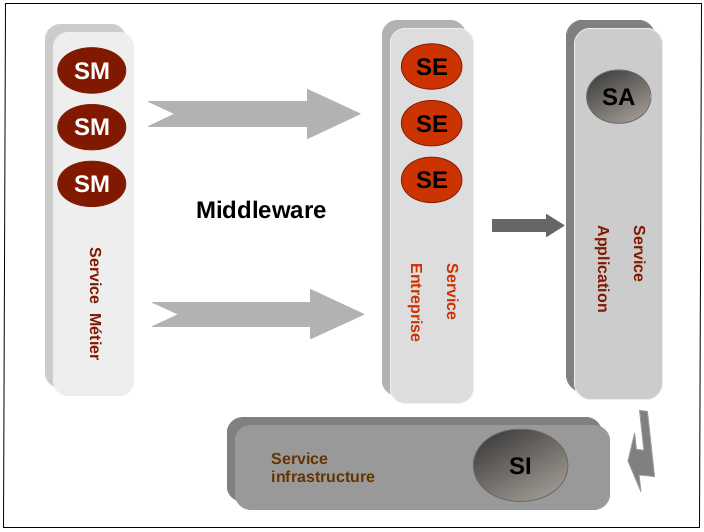
\includegraphics[width=13cm, height=6.8cm]{classif_soa_4.png}
     \captionof{figure}{\textit{Classification Soa}}
     \label{fig4}
   \end{center}
   
   \paragraph{Middleware:} (intergiciel) est un programme qui s'insère entre deux applications et qui va permettre de faire communiquer des machines entre elles, indépendamment de la nature du processeur, du système d'exploitation, voire du langage \cite{refbibMiddle}. \\
   
   Msa est pauvre coté classification, on trouve que deux types/rôles de service comme le montre la figure \ref{fig5}, on aperçoit le service fonctionnel qui encapsule toute la logique métier d'un seul service en une seule brique non partagé et l'infrastructure qui implémente le non fonctionnel (sécurité, logging,..) qui est commun pour les autres services.

   % captures d’écrans 
   \begin{center}
     %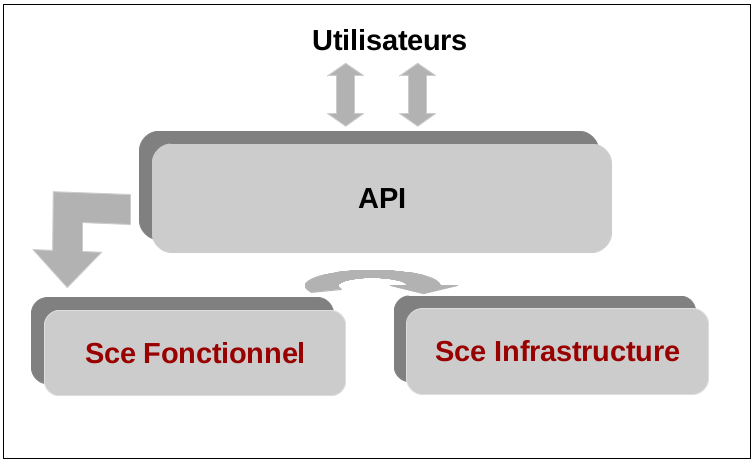
\includegraphics[scale=0.5]{classif_msa_5.png}
     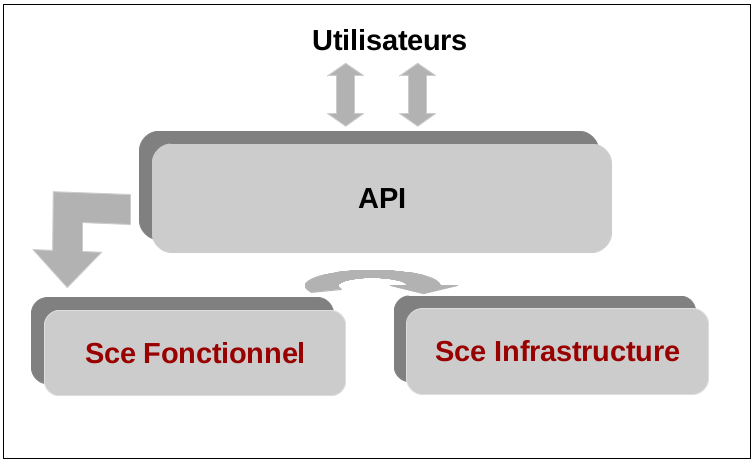
\includegraphics[width=12cm, height=5.5cm]{classif_msa_5.png}
     \captionof{figure}{\textit{Classification microservice}}
     \label{fig5}
   \end{center}
   
  
  \subsection{Structure Organisationnelle} %avant -> détenteur de service
   
   La Structure Organisationnelle des blouses bleus traditionnelle est composée et répartie par spécialité, on trouve des équipes de développement frontend, backend, d'intégration, de testeurs, d'administrateurs de base de données, chacune occupe son espace, cela peut fonctionner et donner ses fruits, néanmoins cette organisation appliquée pour une architecture MS peut avérer mal adéquate et des problèmes vite fais apparaissent, comme qui sera responsable d'un service donné parmi cette structure par équipes, en d'autres termes les MS ont besoins d'un détenteur de service, les ressources humaines ou groupe de l’organisation qui sont responsables de créer et maintenir le service.\\
   
   On a vu au paragraphe précédant la limitation de la classification des MSA(infra, fonctionnel), cela emmène que pour coder ou maintenir un MS il n'est pas nécessaire d'avoir une multitude de groupe de développeur, un groupe pluridisciplinaires est largement suffisant du coût ce service leur appartient et seront responsables du service du début à la fin.
   
    % captures d’écrans 
   \begin{center}
     %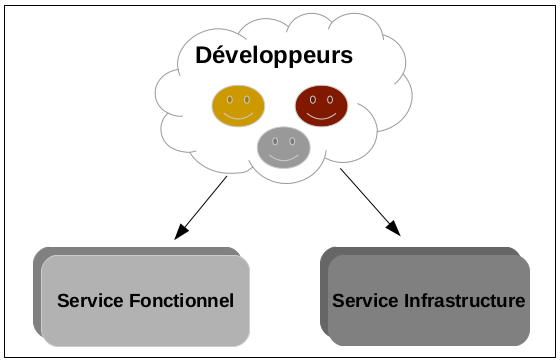
\includegraphics[scale=0.4]{detenteur_service_msa_6.png}
     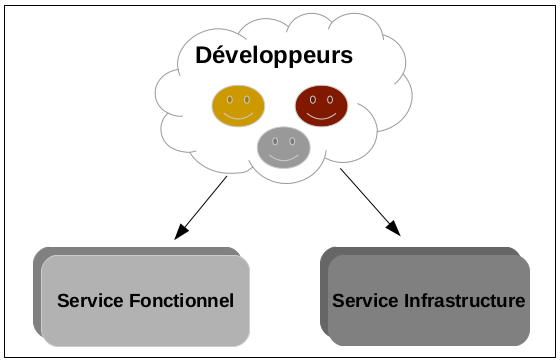
\includegraphics[width=11cm, height=5cm]{detenteur_service_msa_6.png}
     \captionof{figure}{\textit{Détenteur du service en msa}}
     \label{fig6}
   \end{center}
   
   À l'opposé des MSA la ou une variété de classification, ou chaque couche de service appartient à un groupe, il faut en plus de ça l'effort de coordination entre eux, mais avec les MSA y a aucun besoin de coordination et s'il est nécessaire il se fait rapidement à travers d'une même équipe détenteur du service.
   
   Cette différence de la quantité de coordination se répercute directement sur le temps et l'effort nécessaire du développement, build/déploiement, testes et la maintenance du service.
   
   \subsection{Granularité du service}
   Il existe deux concepts clé beaucoup utilisés dans le contexte orienté objet qui permettent de faire des services de qualité issue de GRASP \footnote{General responsibility assignment software patterns} qui caractérise les Msa.
   %itemize
   \begin{itemize}
      \item Forte Cohésion: Favorise la compréhension, la maintenance et la réutilisation des classes qui devront avoir des responsabilités cohérentes spécifique non variées. Une classe est dite faiblement cohésive si elle effectue diverses taches.\cite{refbib5}
      \item Faible Couplage: Le couplage est le niveau de dépendance et d’interaction entre les classes (Composant), on parle de faible couplage lorsque les composants ont peu d’interaction entre eux.\cite{refbib5}
  \end{itemize}
  
  Un MS est petit à fine granularité et expose une fonction qui accomplie une seule tache, implémenté avec un ou deux modules, contrairement aux composants des architectures monolithiques ou distribuées qui ont tendance à grandir offrant une variété de fonctions et de taches parfois implémenter en sous systèmes.
  
  La granularité touche la performance et les transactions. Un service avec une granularité mal conçue, pour accomplir une requête utilisateur consommera un coût de transport élevé entre les appels distant car il aura besoin de relayer et déléguer la tache aux services plus profond. 
  
    % captures d’écrans 
   \begin{center}
     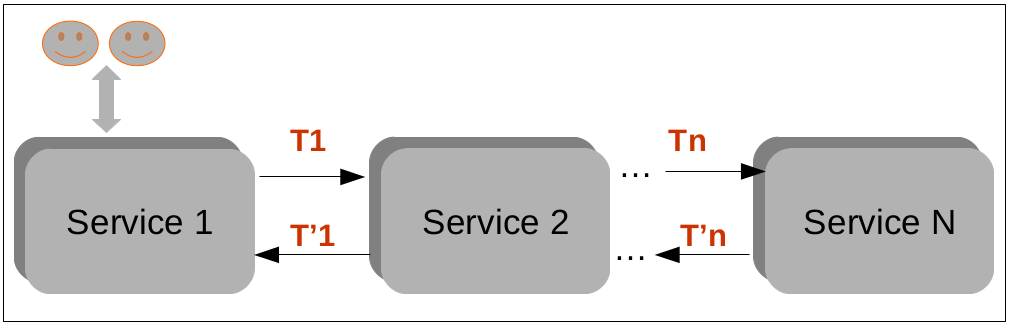
\includegraphics[scale=0.38]{impact_perform_10.png}
     \captionof{figure}{\textit{Impacte sur les performances}}
     \label{fig10}
   \end{center}
   
   La figure \ref{fig10} au dessus illustre un exemple de très fine granularité, pour accomplir une requête utilisateur il faut un temps de transport entre appels distants sans compter le temps de processing qui est T1+T2+...+Tn+T'1+...+T'n (n étant le nombre de service de transite) ce qui est coûteux, la solution consiste à fusionner ces services on un seul pour réduire le coût de transport en T1+T'1.\\
   
    % captures d’écrans 
   \begin{center}
     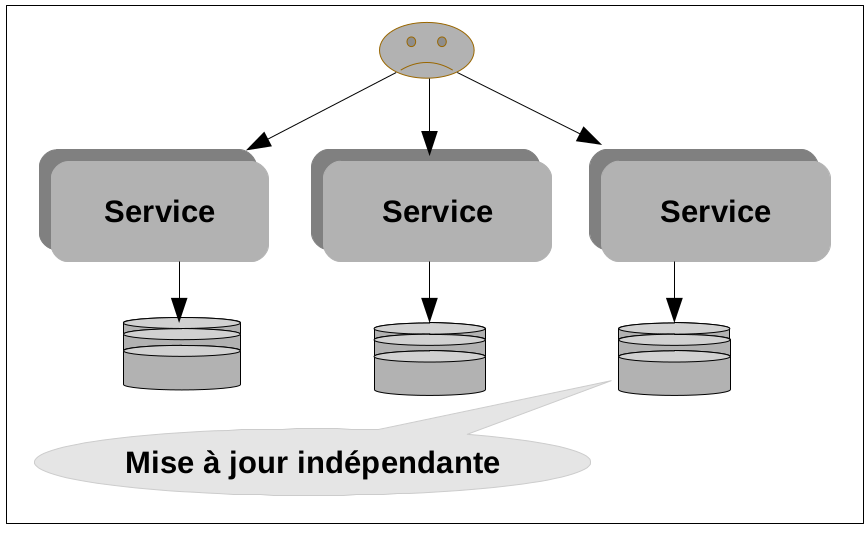
\includegraphics[scale=0.35]{impact_transac_11.png}
     \captionof{figure}{\textit{Impacte sur les transactions 1}}
     \label{fig11}
   \end{center}
   
   Les transactions sont aussi touchées, comme l'illustre la figure \ref{fig11} si il y a une très fine granularité on aura des mises à jour indépendantes dans la base de données du coup ça sera difficile de coordonner le service en utilisant une seule transaction, par contre en fusionnant en un seul service distant, on peut gérer les requêtes engendrer par des mises à jour transactionnelles comme le montre la figure \ref{fig12}.
   
    % captures d’écrans 
   \begin{center}
     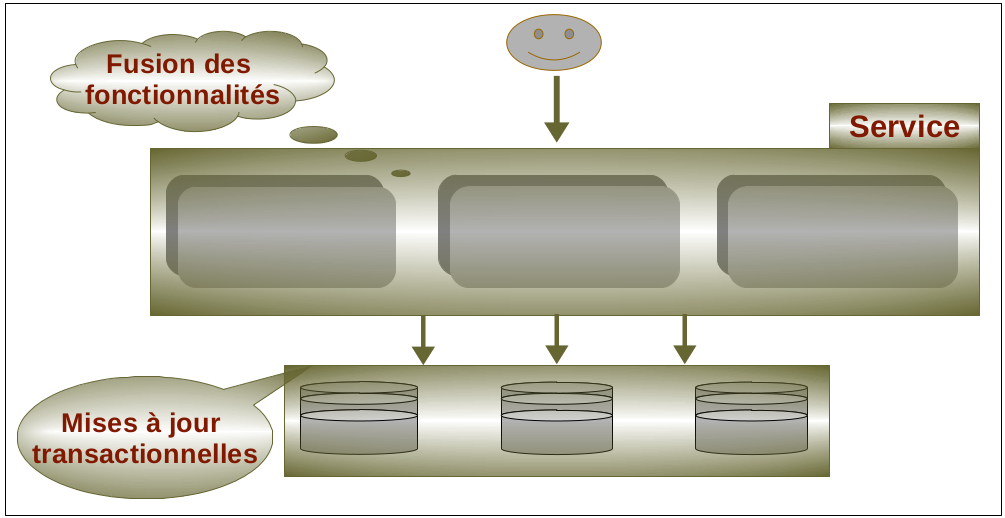
\includegraphics[scale=0.33]{impact_transac_12.png}
     \captionof{figure}{\textit{Impacte sur les transactions 2}}
     \label{fig12}
   \end{center}
   
 \section{Caractéristiques d'architecture}
 
  Dans cette partie on va aborder les briques (composants) architecturales, comment communiquent ils, les composants partagés, et leur accessibilités à partir des services distants ou par les consommateurs.\\
  
   \subsection{Composants partagés}
    Pour illustrer ça, assumons au départ qu'on a devant nous un système de réservation répartie sur trois sous-système: gestion des clients, des réservations et de l'entrepôt de données, figure \ref{fig13}, chacun à sa propre définition de la notion 'réservation', pour une requête client signifie une reproduction de la réservation dans différents sous-système sans compter le travail de coordination.

     % captures d’écrans 
   \begin{center}
     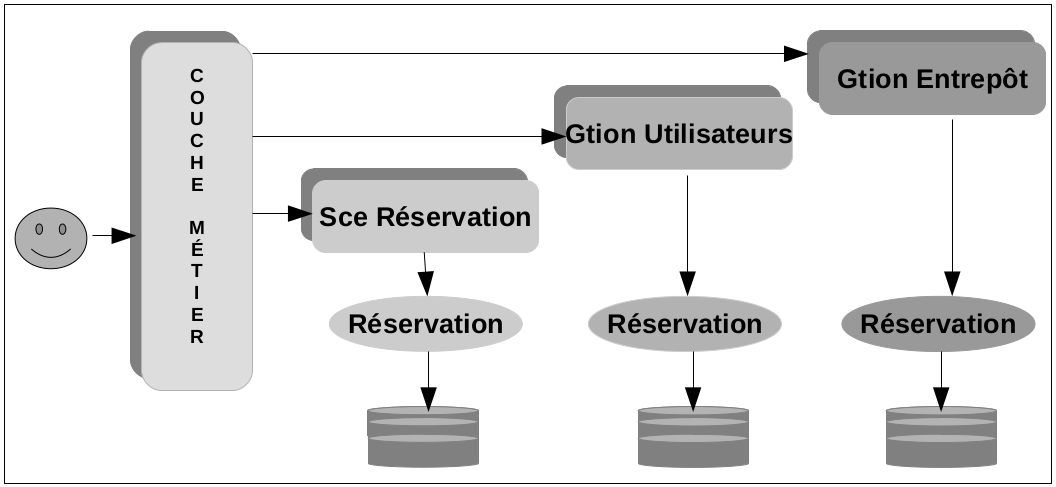
\includegraphics[scale=0.3]{compos_partag1_13.png}
     \captionof{figure}{\textit{Redondance de composants}}
     \label{fig13}
   \end{center}
    
    Cette duplication pousse les architectes à factoriser toute les fonctionnalités qui se ressemble en un seul endroit comme composant partagé du système, si on revient vers notre exemple, on aura un seul travail de 'réservation' partagé entre les trois sous-système, figure \ref{fig14}.
        
   % captures d’écrans 
   \begin{center}
     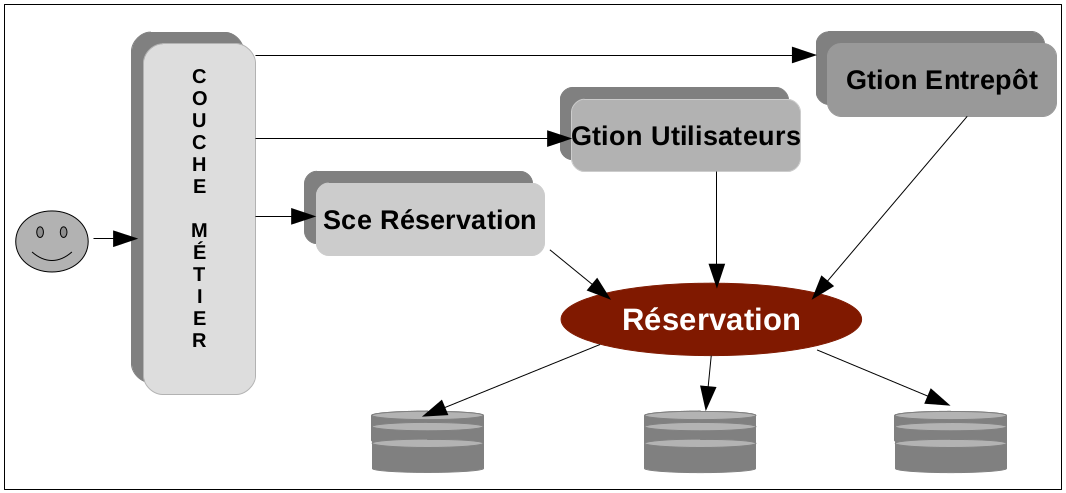
\includegraphics[scale=0.3]{compos_paratag2_14.png}
     \captionof{figure}{\textit{Composants partagés}}
     \label{fig14}
   \end{center}
    
   Les composants partagés est une solution pour factoriser le code des fonctionnalités métier mais, tendent à grandir au fil du temps, ne résous pas la réplication de données, crée un fort couplage et trop de dépendance et ça devient vulnérable aux changements.\\
   
   Les MSA adopte une philosophie qui dit 'partager le moins possible' \cite{refbib6} , avec une encapsulation à la fois des traitements et des données en exposant une interface.\\
   
   Au cours du développement, il apparaît toujours une duplication de code qu'on devra factoriser même avec les MSA comme le service infrastructure, mais contrairement aux autres architectures basées services qui favorisent le maximum de composants partagés, les MSA essaient de partager le minimum possible. Il existe des façons dites brusque pour apparier au partage de composant, c'est la duplication de code des fonctionnalités communes dans chaque MS.\\
   
   
   \subsection{Orchestration et Chorégraphie}
   
    D'abord pour expliquer ces deux notions, on penche au monde de la culture ou je fais référence à la musique et la danse, puis on verra l'impacte de ces notions sur les MSA.\\
    
    Pour faire simple, dans le monde musicale avec un groupe de musiciens (orchestre) qui jouent avec différents instruments, on trouve cet individu avec une baguette à la main qui dirige ou orchestre l'ensemble, afin de produire une musique, c'est de la même façon pour la coordination des services (voir figure \ref{fig15}).\\
     
    J'attribue l'orchestration à la coordination des services à travers un médiateur centralisé pour but d'accomplir un travail métier. \\
     
    % captures d’écrans 
    \begin{center}
      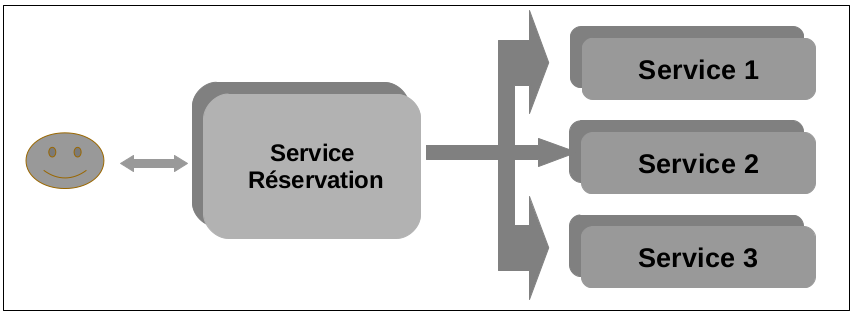
\includegraphics[scale=0.3]{service_orchestra_15.png}
      \captionof{figure}{\textit{Orchestration des services}}
      \label{fig15}
    \end{center}
    
    Laissant le monde musicale et partant vers le domaine de la danse, sur une scène on observe un groupe de danseurs qui bougent et dansent ou chaque individu est synchronisé avec un autre sans qu'il y a un médiateur qui les dirigent.\\
    
    La chorégraphie c'est cet enchaînement et la communication qui se passe entre les services, ou la séquence d'appel d'un service à un autre pour accomplir une tache sans qu'il y est un orchestrateur qui dirige au milieu (voir figure \ref{fig16}).
    
    % captures d’écrans 
    \begin{center}
      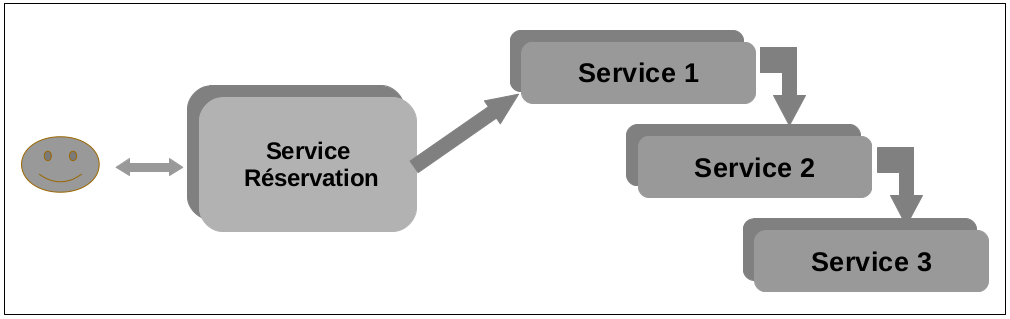
\includegraphics[scale=0.3]{service_choreg_16.png}
      \captionof{figure}{\textit{Chorégraphie des services}}
      \label{fig16}
    \end{center}
    
    Les MSA se basent plutôt sur la chorégraphie que sur l'orchestration cela est due à différentes raisons. La plus importante c'est l'absence du médiateur centrale pour orchestrer, le manque de profondeur dans l'architecture MS aussi joue un rôle comme le montre la figure \ref{fig17}, on constate deux parties essentielles le service lui même et la couche API.\\
    
    NB: sur la figure \ref{fig17} j'ai pas mis en évidence la modélisation non fonctionnelle des service effectuant des taches d’infrastructure. \\
    
    % captures d’écrans 
    \begin{center}
      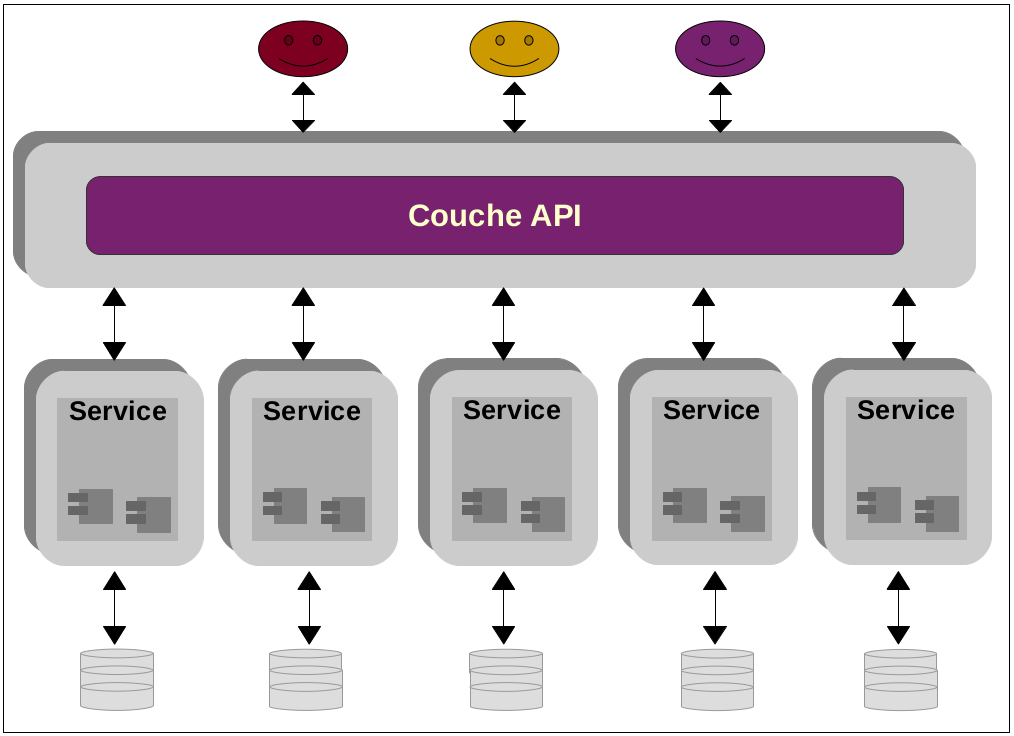
\includegraphics[scale=0.3]{topologie_msa_17.png}
      \captionof{figure}{\textit{Topologie Msa}}
      \label{fig17}
    \end{center}
    
    Les MSA possèdent un minimum de chorégraphie, on trouve pas non plus une longues séquence d'appel d'un service à un autre due au faible couplage/interaction entre services et sa politique 'partager le moins possible' (sauf à l'exception avec l'infrastructure), et si vous sentez à un certain moment le besoin de chorégraphier vos services c'est peut être dû à la très fine granularité de vos fonctionnalités.\\
     
    Trop de chorégraphie engendre un couplage élevé et ça entraîne une mauvaise performance due au temps nécessaire de transport de l'information entre les remotes. 
    
    L'issue pour les longues chorégraphies avec les MSA c'est d'incorporer la fine granularité en grosse granularité. Si une fonctionnalité à fine granularité est partagée par une multitude de service se manifeste, alors soit on l'isole en un MS à part, ou de l'annexer dans chaque MS qui a besoin de cette fonctionnalité en fermant les yeux sur la duplication de code.
   
   La figure \ref{fig18} suivante illustre une modélisation du regroupement de deux service à fine granularité en un service.\\
   
    % captures d’écrans 
    \begin{center}
      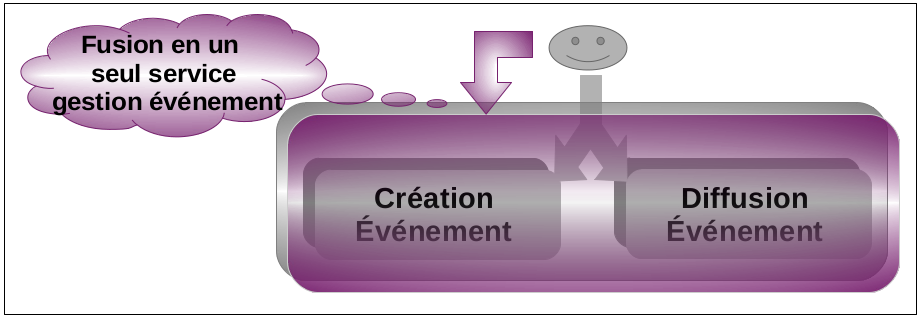
\includegraphics[scale=0.3]{fusion_service_18.png}
      \captionof{figure}{\textit{Exemple de fusion de service}}
      \label{fig18}
    \end{center}
    
    
   \subsection{Communication} % avant -> Couche API
   
    La couche API qui apparaît sur la classification des MSA (figure \ref{fig5}) remplace l'intergiciel (bus) des architectures basées service que les MSA n’implémente pas souvent, cette couche est un service d’accès façade situé entre le service client et le service métier, elle forme une couche d'abstraction et isole, découple le consommateur du micro-service, de cette façon la localisation du MS est ignorée par le client, permet aussi de préserver le service client des changements que le MS subira, du coup on obtient un système qui évolue au fil du temps sans impacter les consommateurs.
    
    Prenons un exemple, supposons qu'on a un service métier à grosse granularité qu'on veut scinder en deux services fins pour des raisons de montée en charge, on est capable de porter des modifications de code du service sans que le client le sache en fractionnant son unique requête vers les deux services engendrer à travers la couche API.\\
    
    Bien que les micro-services peuvent implanter une variété de protocole pour les appels distants et la communication entre eux, le protocole REST est le plus répandu.
    
    Pour réaliser la reconnaissance des services entre eux, chaque service aura besoin de localiser les services dont il a besoin et mettre en place un mécanisme de loadbalancer comme point d'entrée pour gérer la montée en charge et rediriger les requêtes.
    
    Néanmoins, cette solution utilisant une couche API REST avec un loadbalanging semble correcte au cas on a une poignée de service, au cas contraire ça devient difficile de gérer la communication REST à plusieurs raisons, si les services changent de localisation alors une reconfiguration sera nécessaire, la multitude de service engendre l'effet spaghetti, REST est asynchrone. Tout cela induit une convergence vers la lourdeur du système. \\
     
    En s’appuyant sur la couche abstraite API, les MSA perdent certains moyens architecturaux d'entreprise tel que service de messagerie amélioré (EMS Enhanced Messaging Service) et la conversion de message, par contre elles peuvent adopter le service de nommage (annuaire) et la conversion de protocole à une condition.\\
    
    % captures d’écrans 
    \begin{center}
      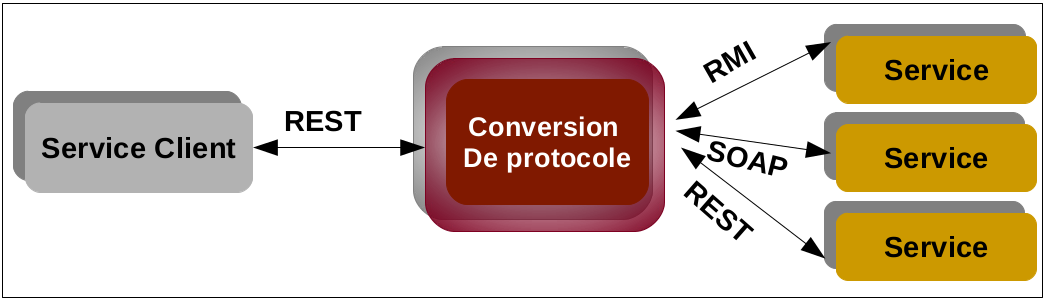
\includegraphics[scale=0.3]{convers_protoco_19.png}
      \captionof{figure}{\textit{Conversion de protocole}}
      \label{fig19}
    \end{center}
    
    La conversion de protocole c'est quand le client effectue un  appel distant avec l'utilisation d'un protocole que le service métier n'attend pas, exemple figure \ref{fig19}. Les MS supportent de multiple types de protocoles,  mais pour faire mieux c'est d'essayer d'utiliser le même protocole. \\
    
    % captures d’écrans 
    \begin{center}
      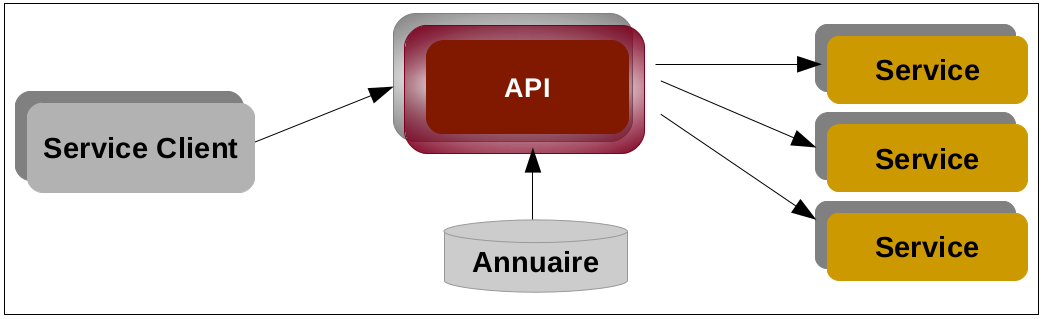
\includegraphics[scale=0.3]{annuaire_20.png}
      \captionof{figure}{\textit{Utilisation du service de nommage}}
      \label{fig20}
    \end{center}
    
    Le service de nommage (annuaire) permet de localiser et d'obtenir un réfèrent du service cible et de l'invoquer (figure \ref{fig20}), Les MS peut utiliser ce paradigme à travers la couche API, ça reste déconseillé car il crée une dépendance de médiateur centralisé.  \\ \\
    
    % captures d’écrans 
    \begin{center}
      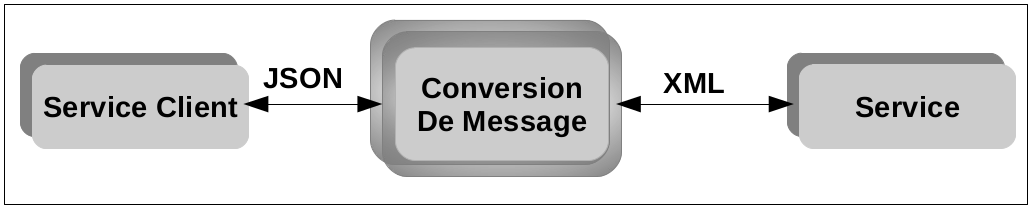
\includegraphics[scale=0.3]{convers_msg_21.png}
      \captionof{figure}{\textit{Conversion de message}}
      \label{fig21}
    \end{center}   
    
    La conversion de message que les MSA n'adoptent pas, c'est la conversion du format des données transmis entre le consommateur et le service métier, la figure \ref{fig21} montre un client faisant appel au service cible en transmettant des données au format JSON alors que le service a besoin des données au format XML.\\
    
   
   L'autre moyen d'intercommunication c'est par bus de messages (figure \ref{fig26}), on a abordé précédemment  que la communication par service REST n'est efficace que si leur nombre est raisonnable avec un faible couplage, avec cette alternative les MS n'ont plus besoin de se localiser.
   
    % captures d’écrans 
    \begin{center}
      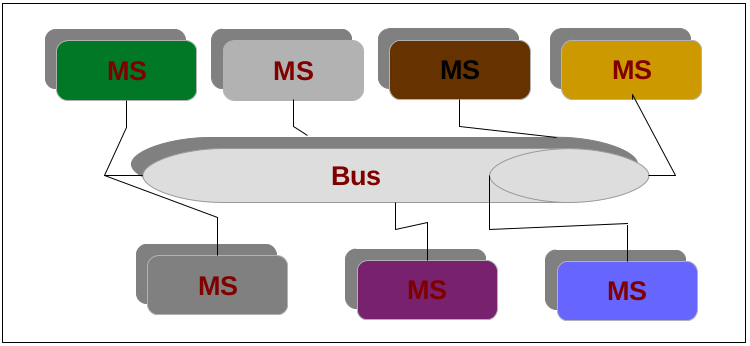
\includegraphics[scale=0.3]{intercomm_msg_26.png}
      \captionof{figure}{\textit{Intercommunication par messages}}
      \label{fig26}
    \end{center} 
   
    L'intercommunication par message fait des services des consommateurs/consommés, les échanges deviennent asynchrone, de ce fait le système sera fluide et facilement scalable, néanmoins une dépendance vers l'infrastructure (bus) n'est pas évitable. 
   
     
%******************Chapitre Comparatif MS**************************** 
\chapter{Étude comparative des principaux framework Micro-service}
 %\markboth{Titre plus court}{Études comparatives des principaux framework Micro-service}
 \chaptermark{Étude comparative}
 
  Dans cette section, nous définissions une liste de quelques frameworks microservices et les éléments de comparaisons puis nous comparerons ces frameworks sur des aspects techniques et non techniques.\\
  
 \section{Frameworks orientés micro-service}
 
  Notre sélection des frameworks micro-service pour mener cette étude est la suivante:
  
    %itemize
   \begin{itemize}
      \item \textbf{Dropwizard}: est un framework Java léger pour développer des micro-services et applications web, son objectif est de fournir des implémentations performantes et fiables de tout ce dont une application web prête à l'emploi a besoin, réduisant à la fois le temps de mise en production et les charges de maintenance.\\
      Site web: \url{http://www.dropwizard.io}
      %\href{http://www.dropwizard.io}{Wikibooks home}
      
      \item \textbf{Spring Boot}: Spring est l'un des frameworks les plus populaires de Java, Spring Boot facilite la création d'applications stand-alone de qualité basées sur Spring, il favorise la convention sur la configuration et est conçu pour vous mettre en route le plus rapidement possible.\\
      Site web: \url{https://projects.spring.io/spring-boot/}
      
      \item \textbf{Vertx}: est un kit d'outils pour la création d'applications réactives sur JVM \footnote{Java virtual machine}, contient plusieurs composants différents conçus pour faciliter l'écriture d'applications réactives et le déploiement de services indépendants dans une gamme de langues différentes destiné à la plate-forme Java \\
      Site web: \url{http://vertx.io/}
      
      \item \textbf{Spark}: Spark est un micro-framework mais très riche en fonctionnalités pour créer des applications web avec un effort minimal. Spark framework est un framework Java simple et léger conçu pour un développement rapide. Il a été inspiré par \textit{Sinatra} \footnote{\url{http://www.sinatrarb.com/}}, un micro framework populaire \textit{Ruby} \footnote{\url{https://www.ruby-lang.org/fr/}}. Ne pas confondre Spark avec \textit{Apache Spark} \footnote{\url{https://spark.apache.org/}}, ce dernier est est un framework Big-Data. \\
      Site web: \url{http://sparkjava.com/}
      
      \item \textbf{WildFly Swarm}:Permet de packager des applications Java EE avec les dépendances minimums sous la forme d’un jar exécutable et autonome que l’on appelle un UberJar ou fat-jar. Celui-ci est déployable grâce à un conteneur embarqué dérivé de Wildfly mais en version minimaliste. Ainsi, chaque fat-jar généré est un microservice léger et déployable, capable d’être scalé de façon indépendante et ne comportant que le nécessaire. \\
      Site web: \url{http://wildfly-swarm.io/}
      
      \item \textbf{Restlet}: Restlet Framework est une solution open source légère, complète destiné à  la plate-forme Java pour développer des API web qui suivent le style d'architecture REST sécurisées et évolutives. Il est disponible pour toutes les plates-formes majeures (Java SE / EE, Google AppEngine, OSGi, GWT, Android) et offre de nombreuses extensions adaptées aux besoins de tous les développeurs. \\
      Site web: \url{https://restlet.com/}
      
   \end{itemize}
   
   
   
 \section{Les éléments de comparaisons}
 
  Dans cette partie, nous définissons les aspects techniques et non techniques de comparaison.
 
  Au début nous comparons notre sélection de frameworks sur des aspects non techniques par rapport à leur licence, langage, version actuelle stable et leur éditeur qu'on a groupé dans une section nommée généralités, puis par rapport à leur communauté, c'est à dire une mesure sur la contribution évolutive pour chacun des frameworks aussi sur leur popularité dans certains sites clés comme \textit{github} et \textit{stackoverflow} .
  
   Par la suite une évaluation sur la documentation, la disponibilité d'information et l'accessibilité au différent frameworks du coté code source et binaires. Jusqu’à la, nos éléments de comparaisons sont classés non techniques.   \\
  
  En dernière analyse, un comparatif technique mettant l'accent sur les serveurs http embarqués par les frameworks, le mécanisme de logging, API Rest et le parseur JSON.\\
 
 \section{Comparaisons}
  
  \subsection{Généralités}
   
   \begin{center}
   \begin{tabular}{|c|c|c|c|c|}
    \hline
    %\rowcolor[rgb]{0.5,0.5,0} \multicolumn{5}{|c|}{Généralités} \\ \hline
    
    \rowcolor[rgb]{0.5,0.5,0}\textbf{Framework} &\textbf{Licence}&\textbf{Langage}&\textbf{Version}&\textbf{Éditeur} \\ \hline
    \textbf{SpringBoot} & Apache License 2.0 & Java & 1.5.6.R & Pivotal \\ \hline
    
    \multirow{6}{*}{\textbf{Vert.x}} &  & Java & 3.4.2 &  \\
                            &  & Scala & 1.1.0-M1 &  \\ 
                            &  Apache License 2.0 & Groovy & 2.1.1-final &  \\
                            & Eclipse Public & Ruby & 3.4.2 & Eclipse \\
                            & License 1.0 & Kotlin & 3.4.2 &  \\
                            &  & Ceylon & 3.4.2 &  \\
                            &  & JavaScript & 3.4.2 &  \\ \hline
                            
    \multirow{2}{*} {\textbf{Dropwizard}} & Apache License 2.0 & Java & 1.1.2 & Coda Hale \\
                                          &  &  &  & Yammer \\ \hline
    
    \multirow{2}{*} {\textbf{Spark}} & Apache License 2.0 & Java & 2.6.0 & Per Wendel \\ 
                            &   & Kotlin & 1.0.0-alpha &  \\ \hline
                            
    \multirow{1}{*} {\textbf{WildFly Swarm}} & Apache License 2.0 & Java & 2017.7.0 &  Red Hat \\ \hline
                            
    \multirow{1}{*} {\textbf{Restlet}} & Apache License 2.0 & Java & 2.3.10 & Noelios \\ \hline
                            
   \end{tabular}
   \captionof{table}{Généralités}
   \label{tab1}
   \end{center}
   
   Spring Boot, Dropwizard, Vert.x, WildFly Swarm, Restlet et Spark utilisent une licence \textit{Apache License 2.0}\footnote{\url{https://www.apache.org/licenses/LICENSE-2.0}}, s'agit bien sûr d'une licence \textit{Libre}\footnote{\url{https://fr.wikipedia.org/wiki/Logiciel_libre}} et \textit{Open Source}\footnote{\url{https://fr.wikipedia.org/wiki/Open_source}} écrite et approuvée par \textit{l'Apache Software Foundation}\footnote{\url{https://www.apache.org/}} en janvier 2004, compatible avec la GNU GPL \footnote{\url{https://www.gnu.org/licenses/gpl.html}}.
   
   Apache License 2.0 autorise la modification et la distribution du codes sous toute forme (libre ou propriétaire, gratuit ou commercial) et plus protectrice à l’égard des brevets et copyright lors de toute modification et compris le texte de la licence elle-même.
   
   Elle est simple à utiliser, il suffit d’inclure une copie de la licence Apache License 2.0 et des messages spécifiant l’utilisation de code sous cette licence qui doivent être déposés dans le répertoire racine de la distribution.
   
   Les messages sous forme d'un document texte qui inclut une notice sur l'utilisation de code sous Licence Apache, le nom des librairies et de leurs développeurs, l'interdiction de supprimer toutes lignes originales sur les copyrights ou brevets soumis à la licence, Un avertissement précisant les modification.
   
   
  
  \subsection{Communauté}
   
     En ce qui concerne le soutien communautaire, des recherches sur ces frameworks sur le web notamment leur dépôt officiel \textbf{github} et \textbf{Stackoverflow}, nous a permis de collecter des données, modélisées sous forme de tableau \ref{tab2} au-dessous, au 22 juillet 2017 . \\  \\
   
   \begin{center}
   \begin{tabular}{|c|c|c|c|c|}
    \hline
    %\rowcolor[rgb]{0.5,0.5,0} \multicolumn{5}{|c|}{Membres de l'équipe} \\ \hline
    
    \rowcolor[rgb]{0.5,0.5,0}\textbf{Framework}&\textbf{Contributeur}&\textbf{commit}&\textbf{Stackoverflow}&\textbf{\% repense} \\ \hline
    
    \textbf{SpringBoot} & 365 & 12.93K & 23.5K & 56\% \\ \hline
     
    \textbf{Dropwizard} & 291 & 4.24K & 1.3K & 61\% \\ \hline
     
     \textbf{Vert.x} & 106 & 2.96K & 759 & 62\%\\ \hline
     
     \textbf{Spark} & 101 & 909 & 352 & 55\% \\ \hline
     
     \textbf{WildFly Swarm} & 73 & 3.291K & 80 & 42\% \\ \hline
     
     \textbf{Restlet} & 39 & 8.536K & 1.240k & 68\% \\ \hline
     
   \end{tabular}
   \captionof{table}{Communauté des frameworks}
   \label{tab2}
   \end{center}
   
   % SB: on 6 Aug 2013 . DW: on 15 Mars 2011 . Vert.x: on 10 Oct 2011 . Spark:  on 7 Feb 2013 
   
   
   Étonnamment, il s'avère que sur StackOverflow, il y a 23 fois plus de sujets sur Spring Boot, que Dropwizard et plus de 30 fois par-rapport à Vert.x et Spark.\\
   Ce n'est pas ce qu'on peut attendre, car Spring Boot est le plus jeune de tous.\\
   
   Le nombre de contributeurs sur Github montre que Spring Boot est au top.
   
   Le nombre de commit et les cycles de livraison de nouvelles versions, favorisent également Spring Boot, ils sont beaucoup plus fréquents avec des petits intervalles, même si Dropwizard, Vert.x et Spark bénéficient d'un excellent soutien de leur communauté, mais leurs cycles de livraison sont lents. De même l'écosystème autour de Spring Boot qui est plus large - il fournit les modules qui permettent l'intégration avec Spring, n'est pas un obstacle pour sa communauté.
   Ce que Dropwizard offre ici, c'est quelques packages d'intégration et beaucoup de projets communautaires.\\
  
   Il semble aussi que la communauté Spring Boot sur Stackoverflow est beaucoup plus réactive aux problèmes des utilisateurs. D'une manière générale, Spring Framework est parrainé par Pivotal, donc il y a beaucoup plus d'activité autour de lui. Dropwizard n'est plus développé par Coda Hale, il a décidé de confier un développement supplémentaire à la charge de sa communauté, ce qui a un impact sur la qualité du support.
   
   
  \subsection{Documentation et accessibilité}
  %creer un tableau: SCM repository ->accé au code, Tutoriels: exemple en ligne, Doc: en ligne, repository Manager publique: mvnrepository, central....
  
   Dans le tableau \ref{tab3} au-dessous sont mis en évidence les différents éléments fournit par les développeurs des frameworks pour leur accessibilité ainsi que leur documentation.\\
   
   \textbf{NB:} \\
    - SCM repository: Source code management repository, c'est le gestionnaire du code source.\\
    - Repository Manager: c'est le gestionnaire des binaires.
   
   \begin{center}
   \begin{tabular}{|c|c|c|c|c|}
    \hline
    
    \rowcolor[rgb]{0.5,0.5,0}\textbf{Framework}&\textbf{SCM repository}&\textbf{Repository Manager}&\textbf{Tutoriels}&\textbf{Doc} \\ \hline
    
    \textbf{SpringBoot} & Github & MvnRepository & Oui & en ligne \\ \hline
     
    \textbf{Dropwizard} & Github & MvnRepository & Oui & en ligne \\ \hline
     
     \textbf{Vert.x} & Github & MvnRepository & Oui & en ligne \\ \hline
     
     \textbf{Spark} & Github & MvnRepository & Oui & en ligne \\ \hline
     
     \textbf{WildFly Swarm} & Github & MvnRepository & Oui & en ligne \\ \hline
     
     \textbf{Restlet} & Github & MvnRepository & Oui & en ligne \\ \hline
     
   \end{tabular}
   \captionof{table}{Documentation et accessibilité}
   \label{tab3}
   \end{center}
   
   Les frameworks présentés ici bénéficient d’une documentation complète sur l’ensemble des outils qu’ils mettent à la disposition du développeur. En effet chacun d’entre eux disposent d’une documentation de toute leurs versions consultable en ligne, des tutoriels ainsi que des exemples pour quiconque veut prendre en main et utiliser son framework.\\
   
   Concernant l’accessibilité de ces frameworks, chacun possède un dépôt officiel publique sur github qui permet de les suivre, visualiser et télécharger le code (tableau \ref{tab4}).
   
   \begin{center}
   \begin{tabular}{|c|c|}
    \hline
    
    \rowcolor[rgb]{0.5,0.5,0}\textbf{Framework}&\textbf{Dépôt github} \\ \hline
    
    \textbf{SpringBoot} & \url{https://github.com/spring-projects/spring-boot} \\ \hline
     
    \textbf{Dropwizard} & \url{https://github.com/dropwizard/dropwizard} \\ \hline
     
     \textbf{Vert.x} & \url{https://github.com/eclipse/vert.x} \\ \hline
     
     \textbf{Spark} & \url{https://github.com/perwendel/spark}  \\ \hline
     
     \textbf{WildFly Swarm} & \url{https://github.com/wildfly-swarm/wildfly-swarm}  \\ \hline
     
     \textbf{Restlet} & \url{https://github.com/restlet/restlet-framework-java}  \\ \hline
     
   \end{tabular}
   \captionof{table}{Dépôts github des frameworks}
   \label{tab4}
   \end{center}
   
   
    Aussi chacun d’entre eux met les binaires à disposition des développeurs dans MvnRepository \footnote{\url{https://mvnrepository.com/}} qui est publique.
   


  \subsection{Aspects techniques}
  
   Le tableau \ref{tab5} au-dessous met en évidence quelques critères de comparaison techniques entre nos différents frameworks micro-services
   
   \begin{center}
   \begin{tabular}{|c|c|c|c|c|}
    \hline
    
    \rowcolor[rgb]{0.5,0.5,0}\textbf{Framework}&\textbf{Serveur}&\textbf{REST Api}&\textbf{Logging} &\textbf{JSON}  \\ \hline
    
    \multirow{4}{*}{\textbf{SpringBoot}} & Tomcat & Spring & Logback&Jackson\\ 
                                        & Jetty & JAX-RS & Log4j, Log4j2&Gson\\ 
                                        & Undertow & Jersey 2 & Slf4j& \\
                                         &  &  & Apache Commons &\\ \hline
     
    \multirow{2}{*}{\textbf{Dropwizard}} & Jetty & Jersey 2 & Logback&Jackson\\ 
                                         &  &  & Slf4j& \\ \hline
     
     \textbf{Vert.x} &non& Vert.x Web & JUL&Jackson\\ \hline
     
     \textbf{Spark} & Jetty & Spark & non&Gson\\ \hline
     
     \multirow{3}{*}{\textbf{WildFly Swarm}} & Wildfly & JAX-RS & JBoss-Logging&Jackson \\ 
                                             &  &  & Logstash&JSON-P \\ 
                                             &  &  & FluentD& \\ \hline
     
     \multirow{2}{*}{\textbf{Restlet}} &Restlet Server& Restlet-API & JDK's logging API&Jackson\\ %Restlet Server
                                        & & JAX-RS & (JULI)& \\ \hline
     
   \end{tabular}
   \captionof{table}{Comparaison des aspects techniques}
   \label{tab5}
   \end{center}
   
   \subsubsection{Serveurs HTTP}
   \textbf{-Spring Boot} supporte Tomcat, Jetty et Undertow comme moteur de servlet. Si vous ne spécifiez aucun conteneur de servlet dans la dépendance de Maven, il prend Tomcat comme serveur par défaut et ajoute la version embarqué du moteur sous forme d'une archive JAR aux bibliothèques. \\
   Spring Boot est plus flexible sur cet aspect et vous laisse configurer les serveurs http préférés à utiliser. Voici la version actuelle du support de conteneurs par Spring Boot:
   
   \begin{center}
   \begin{tabular}{|c|c|c|}
    \hline
    
    \rowcolor[rgb]{0.5,0.5,0}\textbf{Serveur}&\textbf{Version Servlet}&\textbf{Java version} \\ \hline
    
     Tomcat 8 & 3.1  & Java 7 \\ \hline
     
     Tomcat 7 &  3.0 & Java 6 \\ \hline
     
     Jetty 9 & 3.1 & Java 7 \\ \hline
     
     Jetty 8 & 3.0 & Java 6 \\ \hline
     
     Undertow 1.1 & 3.1 & Java 7 \\ \hline
     
   \end{tabular}
   \captionof{table}{Serveurs supportés par Spring Boot}
   \label{tab6}
   \end{center}

   \textbf{-Dropwizard} est plus strict sur l'approche de la convention par rapport à la configuration, il permet au développeur d'applications d'utiliser uniquement Jetty comme conteneur de servlet. Vous n'avez pas le choix de modifier les configurations du serveur. \\
   
   \textbf{-Restlet} n'embarque pas un serveur HTTP ou un conteneur comme tomcat ou jetty, il a nul besoin d'un moteur de servlet ni de l'API servlet. Il possède son propre serveur autonome qui fonctionne sur une pure JVM et qui se lance programmatiquement, l'API Restlet vous donne un contrôle étendu sur le mappage des URI. Il comprend une puissante classe d'annuaire pour gérer les fichiers statiques du serveur de manière similaire à celle du serveur Web Apache.\\

   \begin{lstlisting}
    package fr.uparisx.miage.app.httpserver.restlet;
    import org.restlet.Component;
    import org.restlet.Server;
    import org.restlet.data.Protocol;
    /**
     * @author L Kherbiche
     */
    public static void main(String[] args) throws Exception {
        Component comp = new Component();
        Server httpserver = comp.getServers().add(Protocol.HTTP, 8081);
        httpserver.getContext().getParameters().add("useForwardedForHeader", "true");
        comp.start();  
    }
   \end{lstlisting}   
   
   Par conséquent, l'API Restlet n'a aucune dépendance à l'API Servlet, elle dépend uniquement de Java Standard Edition. Cependant, il est parfaitement possible de déployer une application Restlet dans des serveurs d'applications Java EE ou simplement des conteneursde  Servlet. Ceci est possible à l'aide d'un adaptateur Servlet fourni comme extension, par exemple: connecteurs Eclipse Jetty, AJP.\\
   
   \textbf{-Vert.x} n'inclue pas de conteneur ou de serveur Http embarqué, néanmoins il facilite la création d'un ou plusieurs serveurs HTTP afin que votre application puisse recevoir des requêtes HTTP et cela se fait d'une manière programmatique comme suit:
   \begin{lstlisting}
    package fr.uparisx.miage.app.httpserver.vertx;
    import io.vertx.core.AbstractVerticle;
    import io.vertx.core.http.HttpServer;
    /**
     * @author L Kherbiche
     */
    public class VertxHttpServerVerticle extends AbstractVerticle {

       private HttpServer httpServer = null;
       @Override
       public void start() throws Exception {
           httpServer = vertx.createHttpServer();
           // traitement
           httpServer.listen(8081);
       }
    }
   \end{lstlisting}
   
   
   \textbf{-Spark} par défaut, embarque le conteneur de servlet Jetty, pour exécuter Spark sur un autre serveur web , une implémentation de l'interface
   
    spark.servlet.SparkApplication est nécessaire et le filtre suivant doit être configuré dans le descripteur de déploiement web.xml: \\
   
   \begin{lstlisting}
     <filter>
       <filter-name>SparkFilter</filter-name>
       <filter-class>spark.servlet.SparkFilter</filter-class>
       <init-param>
          <param-name>applicationClass</param-name>
          <param-value>com.company.YourApplication</param-value>
       </init-param>
     </filter>
     <filter-mapping>
       <filter-name>SparkFilter</filter-name>
       <url-pattern>/*</url-pattern>
     </filter-mapping>
   \end{lstlisting}
   
   
   \textbf{-WildFly Swarm}  embarque un conteneur dérivé de Wildfly qui est un serveur d’applications écrit en Java. Il était anciennement appelé JBoss Application Server. Wildfly est basée sur la notion de sous-systèmes que l’on peut ajouter ou enlever selon les besoins. Cela permet d’enlever les fonctionnalités inutiles et ainsi réduire la taille et diminuer la consommation mémoire du serveur.
   
   Un sous-système est un ensemble d’extensions permettant d’étendre le serveur, une extension peut fournir des features comme la gestion de servlet, ce qui rend Wildfly facilement configurable. Par exemple, si l’on souhaite avoir comme extension la gestion de servlet, il suffit de ne laisser que l’extension associée.
   
   Le conteneur peut être instancié d'une manière programmatique, ou si on ne fournie pas le code , alors WildFly Swarm traitera la construction du conteneur et le déploiement ultérieur en mode de commande.\\
   
   \subsubsection{API REST}
   
   \textbf{-Spring Boot} par défaut, utilise ses propres implémentations REST qui est Spring Web MVC plutôt que des spécifications standard. Mais, vous pouvez facilement le configurer pour utiliser les bibliothèques JAX-RS ou Jersey 2. De plus, à partir de la version 1.2.0, Spring Boot a intégré le support pour Jersey 2. \\
   
   \textbf{-Dropwizard} avec ses versions inférieur à 0.8.0 le problème était que cette version était étroitement couplée à la version de Jersey 1.x, qui n'était pas compatible avec JAX-RS. Mais à partir des versions postérieur à 0.8.0 Dropwizard a intégrer Jersey 2 dans le framework. Néanmoins à partir de Dropwizard 0.8.0, il utilise que Jersey 2 par défaut pour l'écriture de des API REST. \\
   
   \textbf{-Restlet} par défaut a son propre standard ou modèle qui facilite les échanges entre applications et/ou exposer des services Web de façon RESTful qui est différent du standard JAX-RS. Le framework utilise une approche différente de celle orientée-annotation de JAX-RS, il utilise plutôt une approche classique orientée-classe.\\
   De Plus, selon cette approche les POJOs métier ne sont plus annoter pour en exposer une API REST. En pratique, la granularité entre ressources REST et objets métier n'est pas la même, pour cela, créer des classes Java pour chaque ressource et que ces classes héritent d'une classe de base (org.restlet.resource.Resource en Restlet).
   
   \begin{center}
   \begin{tabular}{|c|c|c|}
    \hline
    
    \rowcolor[rgb]{0.5,0.5,0}\textbf{Caractéristique}&\textbf{API Restlet}&\textbf{JAX-RS 2.x} \\ \hline
    
     \multirow{2}{*}{\textbf{Style d'API Java}} & Centré ressource \& & Centré POJO \& \\  
                                                & héritage  & annotations \\ \hline
     
     \textbf{Nombre d'annotations} &  5 & 24 \\ \hline
     
     \textbf{Entêtes Http supportés} & 50 & 26 \\ \hline
     
     \textbf{Version Java min} & Java SE 5.0 & Java SE 6.0 \\ \hline
     
   \end{tabular}
   \captionof{table}{Api Restlet vs JAX-RS 2}
   \label{tab6}
   \end{center}
   
   En tous cas, avec les dernières versions du projet Restlet, permettent d’intégrer le standard JAX-RS en incluant des librairies externes, du coût les développeurs ont un accès à ces deux approches qui peuvent même être combinées si besoin.\\
   
   \textbf{-Vert.x} utilise par défaut Vert.x Web pour créer des application Restful et n'est pas compatible avec le standard JAX-RS. \\
   
   \textbf{-Spark} Il est conçu pour les services Web REST et est beaucoup plus simple que les solutions standards Java telles que JAX-RS. L'accent est mis sur la productivité des développeurs, et le framework extrêmement léger fournit juste ce qui est nécessaire et pas plus.\\
   
   \textbf{-WildFly Swarm} WildFly Swarm supporte JAX-RS avec les déploiements .war et .jar, Swarm offre également une intégration native avec Swagger, un outil populaire pour fournir une documentation et une interface utilisateur interactive sur les API RESTful.\\
   
   \subsubsection{Logging}
   
   \textbf{-Spring Boot} prend en charge une grande variété de bibliothèques pour le mécanisme de logging. Il propose Logback, Log4j, Log4j2, Slf4j et Apache Commons logging. Par défaut, spring boot utilise Logback comme implémentations de journalisation.\\

   \textbf{-Dropwizard} prend en charge Logback et Slf4j comme les deux seules bibliothèques pouvant être utilisées pour le mécanisme de journalisation.\\
   
   \textbf{-Restlet} par défaut, s'appuie sur l'API de journalisation du JDK (JULI) pour logger, tracer et debugger son activité en ajoutant un paramètre à la JVM: -Djava.util.logging.config.file="/home/myApp/config/myLogging.properties", qui indique l'emplacement du fichier de configuration des logs. Cependant pour utiliser un autre mécanisme de logging, le développeur doit s'appuyer sur des bibliothèques tierces externes.\\
   
   \textbf{-WildFly Swarm} utilise le systèmes JBoss-Logging qui devrait être inclue comme librairie externe, la journalisation se produit sur la console par défaut.\\
   
   \textbf{-Vert.x} utilise le framework de logging JUL (java.util.logging) livré avec le JDK pour éviter d'utiliser des dépendances supplémentaires. Cependant, il permet d'ajouter une implémentation de logging personnalisé\\
   
   \textbf{-Spark} n'embarque pas un mécanisme de logging.\\

   \textbf{NB:} Logback est le mécanisme de logging le plus préféré à présent. Cependant, logback offre de nombreuses améliorations par rapport à log4j et il existe plusieurs raisons de l'utiliser par-rapport à log4j.\\ \\
   
   
   Pour conclure ce chapitre, nous estimons que Spring Boot est la solution la plus adaptée pour faire des micro-services, car il implémente d'autres fonctionnalités comme l'injection de dépendances, les ORM et aussi il inclue un module de sécurité (Spring security) ce qui est demandé par le monde entreprise. De plus, il semble que la maintenance de composants basés sur Spring Boot soit moins pénible. Nous apprécions également sa popularité, en ce qui concerne le soutien communautaire. Beaucoup de modules utilisés par Spring Boot ont une histoire beaucoup plus longue que le projet lui-même et sont considérés comme stables et mûrs et nous sommes impressionnés par la facilité avec laquelle on a réussi à créer une application avec (voir annexe \ref{annexesb}), néanmoins il y a un coût à mettre qui est le coût de formation et de prise en main.\\
   
   Pour une utilisation académique on peut aller très vite en utilisant Spark Java. C'est léger, rapide et très simple à utiliser. Malheureusement, il manque certaines fonctionnalités par rapport aux autres, mais elles sont facilement ajoutées à l'aide de bibliothèques tierces.

   
  
% *********************** Conclusion *****************
\chapter*{Conclusion}
\addcontentsline{toc}{chapter}{Conclusion}
 
 Prendre une décision d'architecture à appliquer pour créer ou migrer un logiciel est une tâche pas facile, car choisir un style d'architecture pour un système d'information a des effets sur la structure, le cycle de vie du projet et l'organisation de l'entreprise.\\

  L'invention de l'architecture micro-service n'est pas un hasard, en effet c'est pour résoudre les obstacles des architectures antérieures notamment la complexité et l'innovation. La solution de base apporter par les MS est de découper en petit projet indépendant, limiter leur taille avec une petite équipe pluridisciplinaire pour chacun des projets.\\
  
  Découper le domaine métier avec un concept fondamental \textit{partager aussi peu que possible} \cite{refbib6}, pour cela la compréhension du métier est primordiale. La manière de découper n'est pas formelle, il arrive parfois qu'on se trompe en prenant de mauvaises décisions, pour limiter leurs impacts, il faut éviter de fractionner toute à la fois, en commençant de sortir quelques contextes délimités en quelques micro-services indépendants, de cette façon si on se trompe, seulement une petite partie du système qui sera touché.\\
  
  
%********************************* LES ANNEXES ********************
%\appendix
\begin{appendices}
 
  \chapter{Micro-service avec spring boot}
  
  \label{annexesb}Je montre ici la simplicité de créer des micro-services en utilisant le framework Spring Boot.\\
  
  Pour commencer assurer vous d'avoir installer l'outil de build apache Maven ($https://maven.apache.org/download.cgi$)et le JDK-8 d'oracle et bien les configurer dans la variables d’environnement de votre système.\\
  
  La première étape on télécharge un archetype maven avec lequel on va travailler, pour faire ouvrer votre invité de commande ou terminal et taper la commande \textit{mvn archetype:generate -DgroupId=org.apache.maven.archetypes -DartifactId=maven-archetype-quickstart} . \\ 
  
  Cette commande va nous générer un simple projet Java, ensuite on modifie le \textit{pom.xml} qui se trouve à la racine du projet et on ajoute la dépendance Spring boot starter comme suit:
  
\begin{lstlisting}
    <groupId>fr.uparisx.miage</groupId>
    <artifactId>ms-miage</artifactId>
    <version>1.0</version>
    <parent>
        <groupId>org.springframework.boot</groupId>
        <artifactId>spring-boot-starter-parent</artifactId>
        <version>1.5.2.RELEASE</version>
    </parent>
    <dependencies>
        <dependency>
            <groupId>org.springframework.boot</groupId>
            <artifactId>spring-boot-starter-web</artifactId>
        </dependency>
    </dependencies>
    <properties>
        <java.version>1.8</java.version>
    </properties>
    <build>
        <plugins>
            <plugin>
                <groupId>org.springframework.boot</groupId>
                <artifactId>spring-boot-maven-plugin</artifactId>
            </plugin>
        </plugins>
    </build>
\end{lstlisting}
 
 Avant d'aller plus loin on va s'assurer que notre projet est bien configuré, pour cela on va lancer la commande  \textit{mvn clean install} qui va permettre de compiler, packager puis installer notre artefact dans notre dépôt local maven.
 
 Maintenant, on code nos classes java, notre classe principale \textit{ExempleMsApp.java} :
 
\begin{lstlisting}
package fr.uparisx.miage.app;

import java.util.Arrays;
import org.springframework.boot.CommandLineRunner;
import org.springframework.boot.SpringApplication;
import org.springframework.boot.autoconfigure.SpringBootApplication;
import org.springframework.context.ApplicationContext;
import org.springframework.context.annotation.Bean;

/**
 * 
 * @author L Kherbiche
 *
 */
@SpringBootApplication
public class ExempleMsApp {

    public static void main(String[] args) {
        SpringApplication.run(ExempleMsApp.class, args);
    }
}
\end{lstlisting}

 Puis notre REST Controller \textit{MsController.java} qui va nous fournir une chaîne de caractères.
\begin{lstlisting}
package fr.uparisx.miage.ctrl;

import org.springframework.web.bind.annotation.RestController;
import org.springframework.web.bind.annotation.RequestMapping;
/**
 * 
 * @author L Kherbiche
 *
 */
@RestController
public class HelloController {

    @RequestMapping("/")
    public String getSomeCaract() {
        return "une chaine de caracteres";
    }
}
\end{lstlisting}
 
 Il nous reste plus qu'a exécuter notre service \textit{getSomeCaract} en utilisant la commande suivante 
 \textit{mvn clean install \&\& java -jar target/ms-miage-1.0.jar}
 
 Pour voir si ça fonctionne on tape la commande \textit{curl localhost:8080} pour obtenir notre chaîne de caractères 
\textit{une chaine de caracteres}.


\chapter{Construction des microservices} % changer le nom du chapitre -> deploiement des MS
 
 \section{Intégration continue des microservices}
 
   La question à laquelle on va répondre ici, c'est comment on va builder chaque micro-service individuellement et ceux à qui on a porté des modifications de code, pour les déployer sans impacter le reste. \\
  
  De multiples choix de build existent certains sont mieux que les autres, le plus simple consiste à utiliser un seul dépôt de codes, un seul serveur d'IC et un seul build, pour construire tous nos services (figure \ref{fig22}), avec cette maniéré de procéder, si un commit/push d'une ligne de code se fait sur un seul MS, ça provoque le cycle de build (vérification, compilation, testes ...) pour tout les autres, cela prend plus temps qui lui faut car hormis le MS concerné le reste du dépôt est construit inutilement, de plus si il est suivit d'un échec de build toute l’équipe sera pénaliser et ne pourra plus porter d'autre changements jusqu'à ce que la correction soit porter pour continuer. Cette technique de build reste à éviter.\\
  
  % captures d’écrans 
  \begin{center}
    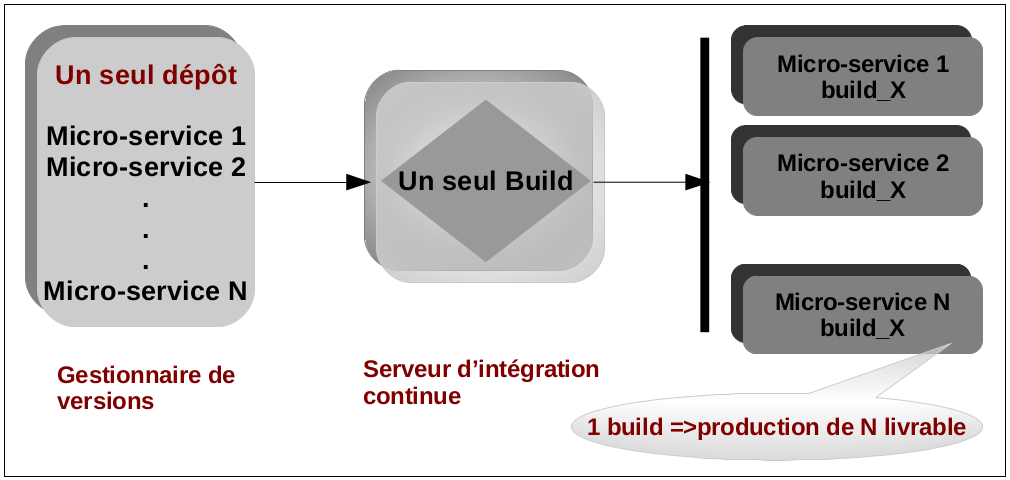
\includegraphics[scale=0.3]{itegra_conti_1_22.png}
    \captionof{figure}{\textit{Build en monobloc}}
    \label{fig22}
  \end{center} 
  
  La démarche de build la plus adéquate pour les micro-services c'est d'avoir une configuration de l’environnement de l'IC permettant de lancer un build par micro-service. Comme le montre la figure \ref{fig23}, chaque MS est construit dans son propre cycle de build séparément du reste.
  
   % captures d’écrans 
  \begin{center}
    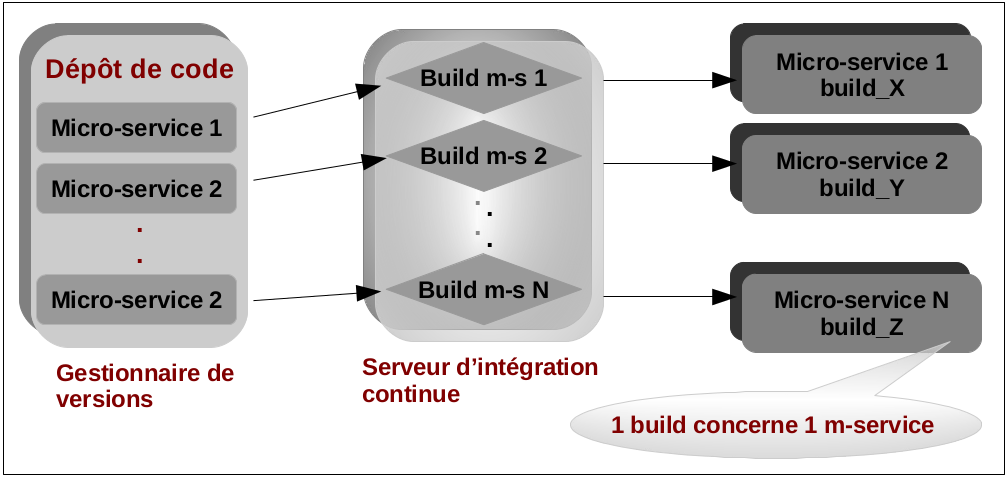
\includegraphics[scale=0.32]{itegra_conti_2_23.png}
    \captionof{figure}{\textit{Un build par micro-service}}
    \label{fig23}
  \end{center} 
 
 Partir du code jusqu'à la prod le MS passe par étapes, le cycle de build (vérification, compilation, testes unitaire...), testes fonctionnels, testes de performances, préproduction puis il passe en production (figure \ref{fig24}), ces étapes font référence à la production continue. \\
 
   % captures d’écrans 
  \begin{center}
    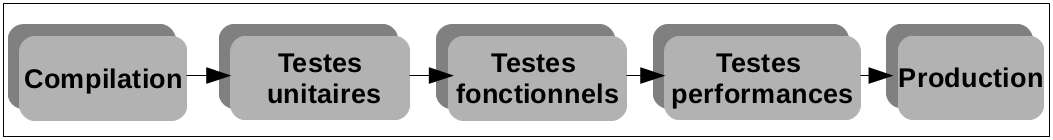
\includegraphics[scale=0.35]{etape_prod_24.png}
    \captionof{figure}{\textit{Modélisation des étapes de production}}
    \label{fig24}
  \end{center} 



\chapter{REST}
  Representational State Transfer  est un style d'architecture pour les systèmes hypermédia distribués, créé par Roy Fielding en 2000 dans le chapitre 5 de sa thèse de doctorat \cite{refbibrest} . Il est devenue très populaire car il offre une alternative des services web SOAP.
  \paragraph{Principes de REST:}
  \begin{itemize}
    \item Interface uniforme: le cœur de REST c'est les ressources, chaque ressource est identifié par une URI Uniform Resource Identifier, les ressources sont séparer de leur représentation, en général avec REST les ressources sont rendues aux client en utilisant un format de données XML ou JSON. En plus la description de la représentation de la ressource encapsule son auto-description, et les interactions entre client et service s'effectue à travers un hypermédia.
    \item Client serveur: avec REST le serveur et le client sont séparés et ont des préoccupations séparé, Cela permet aux deux d'évoluer indépendamment, permet de réduire la complexité et d'offrir de bonne performances. 
    
    \item Stateless: y a pas de sauvegarde de l’état du client au niveau serveur, toute les informations nécessaire pour exécuter une opération sont encapsuler dans la requête.
    
    \item Mise en cache: le serveur peut de gérer les mises en cache en indiquant dans chaque réponse la possibilité de la conserver en cache ou pas incluant des informations concernant sa date de validité et sa date de création. 
      
    \item Système par couche: Étant donné le style de communication entre le client et le serveur, les clients ne connaissent pas spécifiquement le serveur  avec lequel ils interagissent. Ce découplage permet l'introduction de serveurs intermédiaires qui peuvent, par exemple, gérer la sécurité, la monté en charge, la scalabilité .
    
    \item Code on demand: Même s'il fait partie de l'architecture REST, ce principe est facultatif. Les serveurs peuvent transférer du code aux clients pour exécution, cela permet d’alléger le serveur coté traitement.

  \end{itemize}
  
  Pour qu'un service soit considéré comme RESTful, il doit respecter les principes précédents.

\end{appendices}
 
%Bibliographie 
\bibliographystyle{alpha}
\bibliography{biblio}
    
\end{document}